\documentclass{article} % For LaTeX2e
\usepackage{iclr2027_conference}

% Optional math commands from https://github.com/goodfeli/dlbook_notation.
\input{math_commands.tex}

\usepackage{hyperref}
\usepackage{url}
\usepackage{graphicx} % Required for inserting images
\usepackage{longtable}
\usepackage{booktabs} % Professional-looking tables
\usepackage{amsmath,amssymb}
% Keep the ICLR Times family under pdfLaTeX and use its OpenType equivalent
% under XeLaTeX/Tectonic or LuaLaTeX. Load after amsmath/amssymb.
\usepackage{iftex}
\ifPDFTeX
  \usepackage{times}
\else
  \usepackage{fontspec}
  \usepackage{unicode-math}
  \setmainfont{TeX Gyre Termes}
  \setmathfont{TeX Gyre Termes Math}
\fi

% Generated from results_snapshot.json; do not hand-edit.
\newcommand{\StudyBenchmarkCount}{20}
\newcommand{\RetainedCodexCount}{19}
\newcommand{\PrimaryCodexCount}{13}
\newcommand{\VariantCodexCount}{6}
\newcommand{\PaperComparisonCount}{11}
\newcommand{\PaperHigherCount}{7}
\newcommand{\PaperLowerCount}{4}
\newcommand{\PaperEqualCount}{0}
\newcommand{\PaperUnclassifiedCount}{9}
\newcommand{\SuiteHigherPercent}{35.0}
\newcommand{\SuiteLowerPercent}{20.0}
\newcommand{\SuiteUnclassifiedPercent}{45.0}
\newcommand{\PaperHigherPercent}{63.6}
\newcommand{\PaperLowerPercent}{36.4}


% \todo{...} marks a number or claim that is not yet settled. Every one must be
% resolved or deleted before submission; grep for "todo" and for "TODO:" keys.
\usepackage{xcolor}
\newcommand{\todo}[1]{\textcolor{red}{[#1]}}

\title{Beyond Code:\\ When Do Coding Agents Rival Domain Specialists?}

\author{Anonymous authors}

% Show authors in this working draft; comment out for anonymous review.
\iclrfinalcopy

\begin{document}

\maketitle
\ificlrfinal
  \lhead{Working draft}
\fi

\begin{abstract}
% Abstract body. Included by main.tex.
% Registration draft: percentages are displayed without TODO markup; final validation is pending.
% In particular, the provisional 45% on-par group remains unclassified in the source data.
Coding agents are performing exceptionally well on coding benchmarks, but how well their capabilities transfer to inherently non-coding tasks remains unclear. We present an in-depth empirical study of a general-purpose coding agent, Codex, against domain-specific state-of-the-art systems, building a suite of 20 non-coding benchmarks spanning finance, clinical diagnosis, operations research, long-context aggregation, information retrieval, and open-ended scientific research. To make these comparisons rigorous and reproducible, we develop a reusable, AI-assisted meta-analysis pipeline that (1) identifies benchmark-specific state-of-the-art systems and verifies their reported results against primary sources, (2) translates benchmark protocols into executable tasks and audits alignment in instances, metrics, tools, and model configurations, and (3) reproduces specialized systems on a shared backbone and analyzes both agents’ execution traces. We find that Codex outperforms domain-specific systems on 35\% of benchmarks, underperforms on 20\%, and performs on par on 45\%. Our analysis reveals three recurring findings: more complex workflows do not necessarily improve accuracy; task decomposition can lose critical information; and domain-specific scaffolding adds value when it explicitly enforces domain conventions, preserves task conditions, or introduces targeted verification steps that direct Codex may otherwise skip. Codex’s advantage often comes from broader context retention and direct computation rather than pipeline depth, while its characteristic failures more often occur in answer delivery than in intermediate reasoning. Together, the study provides initial evidence of coding agents’ capabilities beyond software tasks and a reviewable evaluation pipeline for establishing when domain-specific scaffolding adds value.

\end{abstract}

\section{Introduction}
\label{sec:intro}

Coding agents combine language-model reasoning with a shell, a filesystem, and the ability to
write and execute programs. These capabilities could also support tasks whose goal is not
software development: diagnosing a rare disease, formulating an optimization problem, finding
evidence in a large corpus, or analyzing scientific data. Domain-specific systems address these
tasks through specialized retrieval, tools, memory, and workflows. When does a general coding
agent rival those systems, and when does domain-specific structure still help?

We study this question using Codex on a suite of \StudyBenchmarkCount{} non-coding benchmarks selected from
554 candidate benchmark records. The collection spans 33 overlapping domain labels and includes
an 83-entry evidence shortlist and a 30-task feasibility-review inventory, each subject to
further selection. SSTQA replaces LongBench v2 in the study suite because the selected DeLM
implementation for LongBench v2 is unavailable; the earlier LongBench measurement remains
in the supplementary results. We incorporate the available reruns and distinguish primary
settings from scored variants throughout. The resulting
suite covers clinical and biomedical reasoning, chemistry and materials science, operations
research, financial and tabular reasoning, retrieval, long-context aggregation, and scientific
research. This breadth makes it possible to examine differences across task types rather than
treat generalization beyond coding as a single score.

\begin{figure}[t]
  \centering
  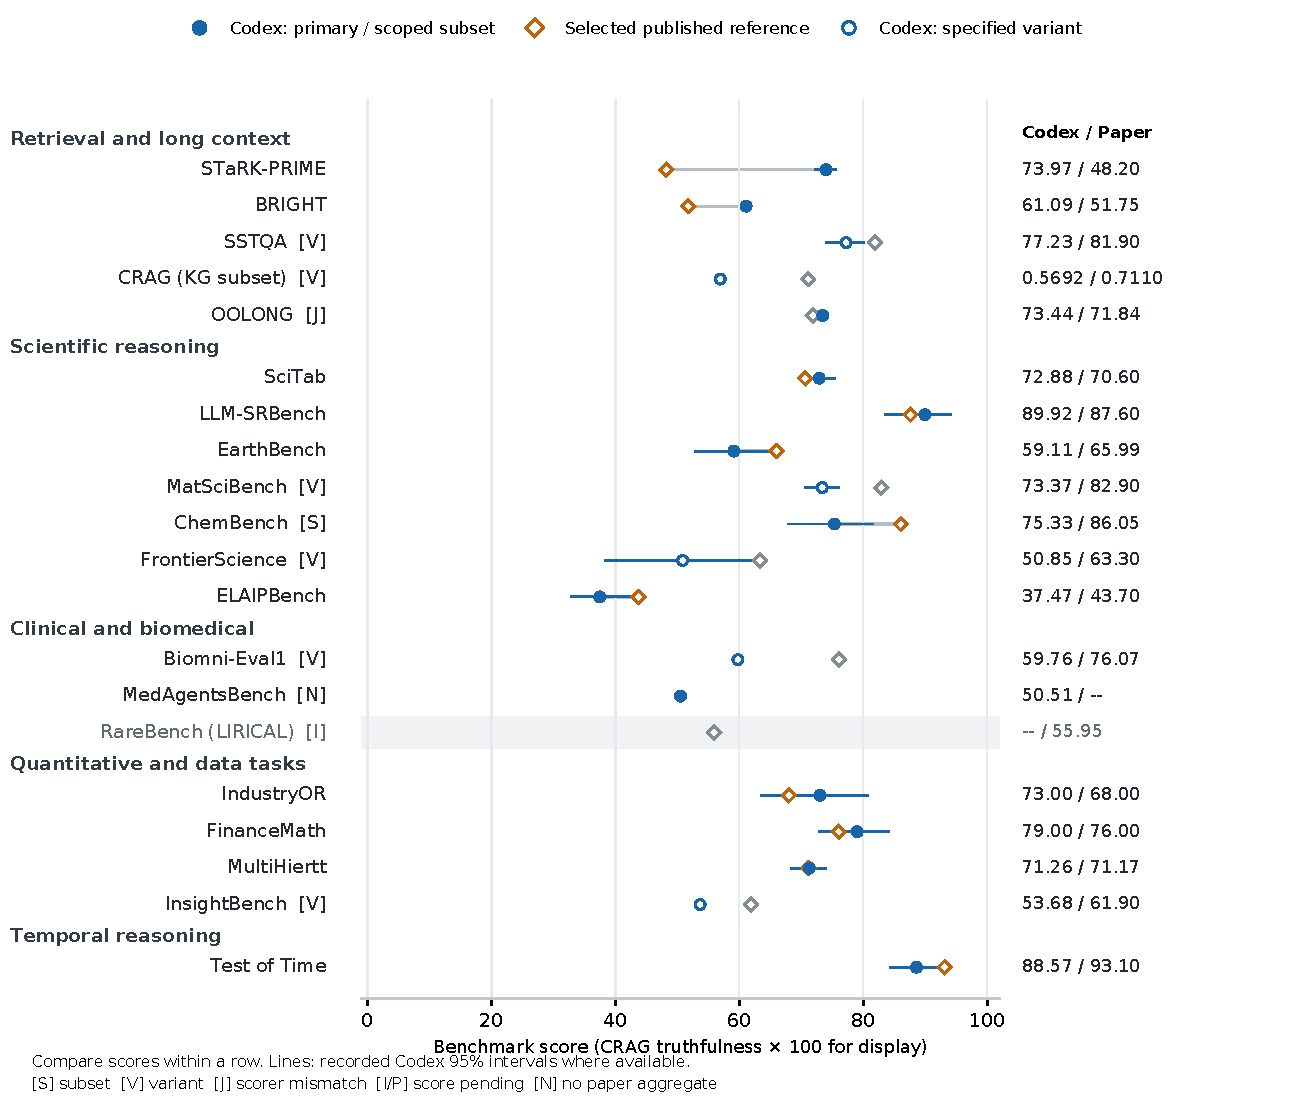
\includegraphics[width=\textwidth]{figures/direct_codex_vs_published.pdf}
  \caption{Direct Codex and selected published reference scores after the HF result refresh.
  Filled circles show primary settings or declared planned subsets; open circles show scored
  protocol variants. ChemBench uses a 150-question open-web pilot; SSTQA shows the English-split
  judge variant, with its Chinese-split primary result pending. RareBench awaits a valid
  network-enabled run. Each row uses its own
  metric (CRAG truthfulness is multiplied by 100 for plotting).
  Appendix~\ref{app:result-details} records coverage, variants, and score provenance. Lines between
  systems mark descriptive paper comparisons, which include backbone and protocol differences.}
  \label{fig:main-results}
\end{figure}

\paragraph{Two complementary comparisons.}
Figure~\ref{fig:main-results} gives the broad comparison with scores reported in the literature.
It answers how the measured coding agent relates to existing reported performance, while retaining
each reference's model and evaluation setting. To examine the contribution of a scaffold, we also
execute specialized systems on a shared backbone and score both arms on the same instances.
These comparisons answer different questions: a gain over a published score may reflect a
stronger backbone, while a shared-backbone comparison more directly tests the system around it.
Reasoning effort, tool permissions, evaluator, and dataset version must still be checked.

\paragraph{A reusable benchmark audit pipeline.}
Establishing either comparison requires identifying the correct reference system, tracing its
score to a primary source, and translating its evaluation protocol into executable tasks.
Our AI-assisted pipeline records these steps as benchmark specifications, run contracts,
declared patches, and auditable evidence (Figure~\ref{fig:audit-pipeline}). It also exposes
limitations of the available benchmark ecosystem: unavailable resources, ambiguous metrics,
changes in answer keys, and differences between a released implementation and its reported
system. These are findings about evaluation design and reproducibility. They are kept separate
from explanations of why one agent solves a task better than another.

\paragraph{Contributions.}
We contribute (1) a broad audit of 554 candidate benchmark records and an evaluation
suite supporting a study covering \StudyBenchmarkCount{} non-coding benchmarks; (2) a reusable pipeline for
finding published reference systems, validating executable evaluations, and documenting the
conditions of comparison; and (3) an empirical comparison organized around experimental rigor,
domain-level performance differences, and the mechanisms behind successes and failures.
Available measurements are included in this draft. The 25\%-subset comparator campaign and
the remaining paired trace analyses are in progress, with unfinished results explicitly marked.

The study evaluates one Codex configuration, not the population of coding agents. Its benchmark
collection is a documented, AI-assisted meta-analysis rather than an exhaustive systematic
review, and its heterogeneous metrics are not pooled into a single performance average.

\section{Related Work}
\label{sec:related}

\paragraph{Coding agents beyond software development.}
SWE-agent studies interfaces for repository navigation, code editing, and execution
\citep{yang2024sweagent}, while OpenHands provides a platform for agents that act through
code, a command line, and a browser \citep{wang2025openhands}. SWE-bench evaluates issue
resolution in real software repositories \citep{jimenez2024swebench}. Beyond software,
GAIA and AgentBench assess information gathering, tool use, and interaction with diverse
environments \citep{mialon2024gaia,liu2024agentbench}; ScienceAgentBench and MLE-bench
evaluate scientific data analysis and machine-learning engineering
\citep{chen2025scienceagentbench,chan2025mlebench}. These studies establish that agent
evaluation extends beyond code generation. Our focus is the transfer of a general-purpose
coding agent to tasks whose target outputs are non-coding, compared with domain specialists
using both published scores and executions on a shared backbone.

\paragraph{Domain-specific scaffolding.}
AutoGen supports multi-agent conversations \citep{wu2024autogen}; DSPy and AFlow optimize
language-model pipelines and agentic workflows \citep{khattab2024dspy,zhang2025aflow}.
Domain-focused systems instantiate this structure through medical expert discussions in
MedAgents \citep{tang2024medagents} and chemistry tool libraries in ChemCrow
\citep{bran2024chemcrow}. Additional structure also creates failure points: MAST organizes
observed multi-agent failures into system design, inter-agent misalignment, and task
verification categories \citep{cemri2025mast}. Building on these perspectives, we examine
whether longer workflows improve accuracy, whether decomposition preserves necessary
information, and when explicit domain conventions, task conditions, or verification help.
Our paired comparisons distinguish published performance from performance on our backbone;
trace examples motivate mechanisms whose causal effects require targeted ablations.

\paragraph{Reliable benchmark evaluation.}
GSM1k probes overfitting to a widely used reasoning benchmark \citep{zhang2024gsm1k}, and
prompt-format experiments show that meaning-preserving changes can alter measured performance
\citep{sclar2024format}. HELM standardizes evaluation conditions across scenarios and metrics
\citep{liang2023helm}, while the Language Model Evaluation Harness provides reusable task
and scoring implementations \citep{gao2023harness}. The NeurIPS reproducibility program
complements such infrastructure with code, checklists, and independent reproduction
\citep{pineau2021reproducibility}. Our audit connects each published score to its reference
implementation and the executable task used for comparison, checking instances, metrics,
answer keys, judges, and resources. These checks establish the conditions for interpreting
performance gaps; we treat them separately from findings about agent capabilities.

\paragraph{AI-assisted evidence synthesis.}
ASReview demonstrates how active learning can prioritize literature screening while retaining
a transparent review process \citep{vandeschoot2021asreview}. Our \emph{meta-analysis pipeline}
extends evidence collection to checking reported benchmark results and executing comparisons.
It does not estimate a pooled effect across heterogeneous metrics, and it is not an exhaustive
systematic review: the search was not preregistered and screening was not performed by two
independent human reviewers. Source records, adversarial checks, and human adjudication make
the process reviewable; an independent accuracy evaluation of the SOTA finder remains
unfinished (Section~\ref{sec:rigor}).

\section{Benchmark audit and evaluation protocol}
\label{sec:method}

We select a suite of \StudyBenchmarkCount{} non-coding benchmarks from 554 candidates and use an AI-assisted audit
pipeline to establish the task, the published reference system, and the conditions of each
comparison (Figure~\ref{fig:audit-pipeline}). The study has two complementary comparisons.
\emph{Direct Codex versus published SOTA} measures performance against the selected system's
paper-reported score; it may combine differences in backbone, scaffold, and evaluation conditions.
\emph{Shared-backbone evaluation} re-runs available specialist systems on our model endpoint to
study the contribution of their scaffolds, with remaining protocol differences declared.
The first comparison supplies Figure~\ref{fig:main-results}; the second requires completed,
audited comparator runs. The comparator evaluations on the 25\% subsets are still running;
unavailable results remain \todo{pending}.

\begin{figure}[t]
\centering
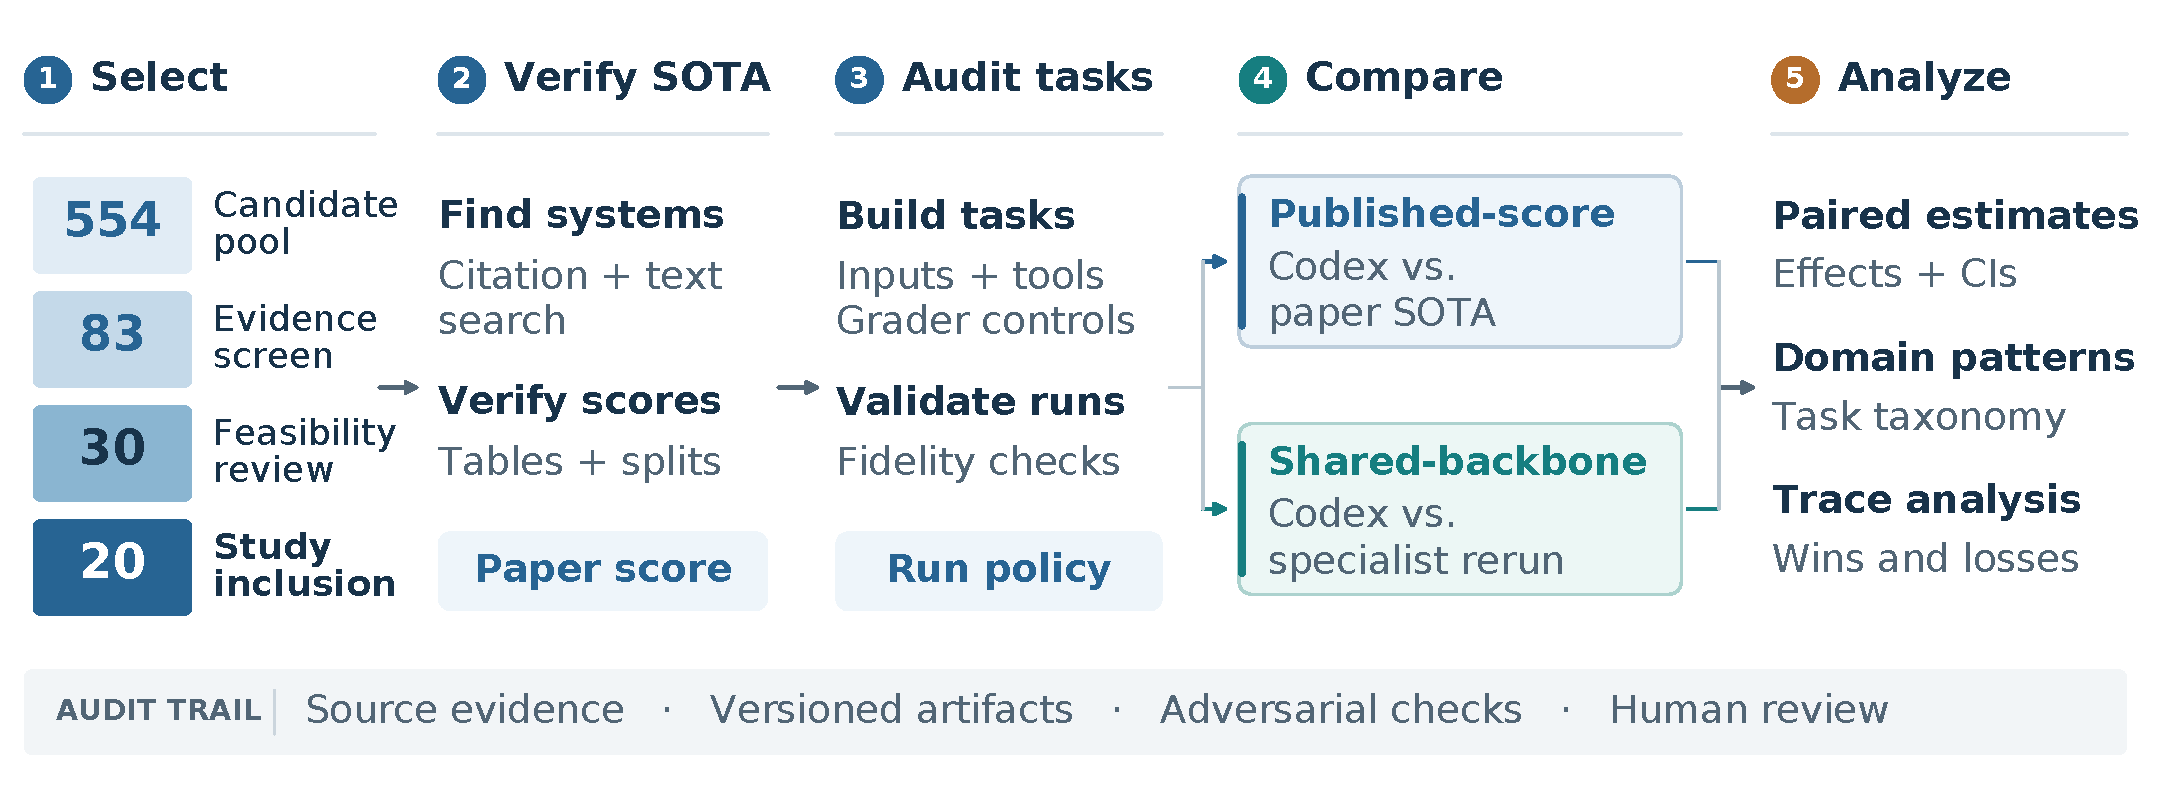
\includegraphics[width=\textwidth]{figures/benchmark_audit_pipeline.pdf}
\caption{The benchmark audit pipeline. Each stage produces reviewable evidence. Published-score
comparisons and shared-backbone re-runs answer different questions; the final stage includes
ongoing comparator evaluations and planned trace analyses. Selection reviews comparator evidence,
non-coding scope, practical testability, and task/protocol fidelity. The counts mark archived
screening checkpoints (Table~\ref{tab:funnel}); they do not denote execution readiness or completed
comparisons.}
\label{fig:audit-pipeline}
\end{figure}

\subsection{Candidate screening and suite construction}
\label{sec:method:collection}

The candidate audit covers 554 benchmarks with 33 overlapping domain labels, including coding
benchmarks that are excluded from the study's non-coding scope. Ordered gates assess scope,
external adoption, comparator availability, reproducibility, and saturation. Benchmarks whose only
reported comparator comes from their defining paper are retained with an
\texttt{author\_reported\_only} flag. Aggregators overlapping separately listed benchmarks are
flagged to avoid double-counting. The evidence tiers distinguish reproducible agent systems,
limited reproducibility or headroom, bare-model reference systems, and excluded cases; they are
screening aids, not estimates of benchmark quality.

Models extract semantic fields from source text; deterministic rules derive tiers from those
fields. Exclusion-relevant labels require source quotations whose presence is checked by code.
Unverified labels become \texttt{unknown} and cannot demote a benchmark, while unverified scores
cannot promote it. Selection also reviews access to data and environments, automated grading,
task fidelity, and the intended comparison frame. A candidate can enter a shortlist or acquire
a task implementation while still requiring resolution of these conditions. Table~\ref{tab:funnel}
records the available checkpoints in this review. The current \StudyBenchmarkCount{}-benchmark
roster replaces LongBench-v2 with SSTQA because DeLM's evaluation code is unreleased;
LongBench-v2's existing measurement is retained in Appendix~\ref{app:supplementary-results}.
Consequently, the suite supports an empirical study of these \StudyBenchmarkCount{}
benchmarks, rather than a representative estimate over all non-coding tasks. Appendix~\ref{app:collection}
gives the screening details and historical tier counts.

\begin{table}[t]
\centering
\small
\begin{tabular}{@{}lrp{0.64\textwidth}@{}}
\toprule
Review checkpoint & $n$ & Selection conditions under review \\
\midrule
Candidate pool & 554 & Benchmark identity, domain, source records, and overlap with other candidates \\
Evidence screen & 83 & Comparator evidence, reproducibility, and headroom; the archived shortlist is an input to further review \\
Feasibility review & 30 & Non-coding scope, data/environment access, automated grading, and task fidelity; a task implementation does not close these checks \\
Study inclusion & \StudyBenchmarkCount{} & Study scope, evaluation-frame review, and run evidence; current inventory retains declared variants and pending cases separately \\
\bottomrule
\end{tabular}
\caption{Selection checkpoints and the conditions examined. The 83-entry shortlist and 30-task
inventory are historical artifacts; their memberships have not yet been reconciled into a frozen,
nested inclusion/exclusion ledger (Appendix~\ref{app:collection}). The updated study inventory
contains \StudyBenchmarkCount{} benchmarks.
\RetainedCodexCount{} have retained scores (\PrimaryCodexCount{} primary/scoped settings and
\VariantCodexCount{} scored protocol variants); RareBench awaits a valid rerun.
These counts do not imply completed paired comparator evaluations.}
\label{tab:funnel}
\end{table}

\subsection{Identifying and verifying published SOTA}
\label{sec:method:opponent}

For each benchmark, we retrieve citing papers through Semantic Scholar and OpenAlex, supplement
citation search with full-text benchmark-name search, and deduplicate by paper identifier
\citep{kinney2023semantic,priem2022openalex}. Models extract candidate results and revisit
low-confidence records and records that would establish SOTA. The selected reference is checked
against its primary-source table and, where available, a maintained leaderboard; an adversarial
search attempts to find a stronger result.

A result is indexed by method, backbone, and evaluation frame: metric, split, instance count,
settings, and source date. We distinguish the best verified score in the target frame from the
best score in any frame, and record agent, bare-model, and classical-system results separately.
Differences in denominators or aggregation cannot be resolved by selecting the larger number.
This procedure creates an auditable reference; it does not establish that search found every
eligible system. Finder accuracy requires a separately adjudicated reference set and remains
\todo{to be measured} (Section~\ref{sec:experiments}).

\subsection{Executable tasks and direct-Codex setup}
\label{sec:method:executable}
\label{sec:setup}

Each benchmark is translated into containerized tasks with instructions, inputs, a pinned
environment, and an evaluator \citep{harbor2026}. The agent phase excludes
gold answers and sibling results; grading occurs separately. Checks cover task manifests, input
delivery, correct-answer and no-action controls, model connectivity, execution validity, and
aggregation. A constant-answer baseline measures how much credit is available without solving
the task. Infrastructure failures are tracked separately from graded incorrect answers.
Task-fidelity declarations record changes to search space, environment, required outputs, and
scope.

Direct Codex uses endpoint \texttt{azure/gpt-5.6-sol}, reasoning effort \texttt{medium}, and one
attempt by default, without an intended benchmark-specific scaffold \citep{openai2026codex}.
CLI versions are recorded per run. The baseline receives the benchmark's own provided or
permitted resources, explicitly named in the prompt: for example, CRAG's mock API, Biomni's
E1 environment, a staged corpus, or permitted public web search. This protocol was fixed in the
2026-09-12 experiment design. Earlier runs that withhold required resources are labeled
\emph{restricted variants} and cannot serve as the benchmark's baseline result. The audit checks
container egress, provider-side search, and task wording separately; open-web runs additionally
require trajectory scans for benchmark gold sources. Appendix~\ref{app:codex-setup} records the
setup and unresolved settings; Appendix~\ref{app:execution} details the checks.

\subsection{Shared-backbone comparison and alignment audit}
\label{sec:method:alignment}

A specialist comparator retains its published scaffold and method-specific components while its
adapter runs against the shared model endpoint. Resources provided or permitted by the benchmark
belong in the baseline; an index, learned embedding, cache, or planner built by the comparator's
authors remains part of that method. Declared tool asymmetries make a reference a
\emph{one-directional bar}: matching or exceeding it is admissible evidence, while falling short
cannot be classified as a Codex loss. Deployment and backbone-substitution patches are declared.
The optional reference-informed arm adds the comparator's paper and scrubbed code to Codex's
baseline; it asks whether Codex can use the described method. Neither adaptation is an exact
reproduction of the original paper configuration.

A per-benchmark \texttt{run\_policy.json} binds the instance set, score definition, tools, sampling,
budgets, published reference, and comparator code version. A comparator's \texttt{alignment.json}
records ten axes against the named reference arm: instances, answer key, grader, backbone,
reasoning effort, sampling, execution environment, network policy, tool access, and compute
budget. Each axis includes the values on both sides, evidence, and an equality or deviation
status. A schema checker verifies completeness; a separate code audit checks whether the
statements are true. An auditor and an adversarial verifier inspect each binding.

Shared backbone alone does not guarantee a controlled comparison. Historical runs can differ in
effort, sampling, answer channel, or available tools; later repaired runs supersede them only when
validated. We retain the relevant caveats beside scores and require common instance IDs for
paired comparisons. Section~\ref{sec:audit} presents the dated alignment findings;
Appendix~\ref{app:alignment} documents the current protocol, including fixed approximately
25\% evaluation subsets drawn with seed 20260917 and benchmark-specific strata. The ongoing
subset runs will be added after completion and validation.

\subsection{Trace analysis and human review}
\label{sec:method:human}

The analysis asks where performance differs by domain, why a specialist outperforms Codex, and
why Codex outperforms a specialist. Execution traces provide evidence about retrieval, task
representation, verification, and recovery; a trace-supported explanation is distinguished from
a causal claim requiring a controlled intervention. Proposed mechanisms without completed trace
comparisons or ablations remain \todo{pending trace analysis}. Instruction, extraction, and
execution defects are reported as measurement and reproducibility findings, rather than as
substantive explanations of domain expertise.

Humans review benchmark identity, reference selection, and unresolved protocol choices through
row-level evidence and a decision register. A comparability ledger records admissibility rulings;
a failure log records pipeline errors and their fixes. Findings become changes to the versioned
pipeline so that affected records can be recomputed. Appendix~\ref{app:review} describes these
review artifacts. The workflow is an AI-assisted meta-review, with the coverage limitations
discussed in Section~\ref{sec:related}.

\section{Experiments}
\label{sec:experiments}

We first establish measurement fidelity, then compare direct Codex with published specialized
systems and with their shared-backbone reproductions. The trace analysis follows the three
findings in the abstract: whether additional workflow stages improve accuracy, how decomposition
preserves or loses information, and when domain conventions, task conditions, and targeted
verification help specialized systems. Figure~\ref{fig:main-results}
summarizes \StudyBenchmarkCount{} benchmark records after checking the current HF branches
on 2026-09-18. Published-reference eligibility, scored Codex variants, and paired-comparator
completion are recorded separately. Ongoing comparator
runs evaluate fixed 25\% subsets; their unfinished results remain \todo{pending}.
The Codex configuration and per-benchmark operating conditions are given in
Section~\ref{sec:setup} and Appendix~\ref{app:codex-setup}.

\subsection{Experimental rigor}
\label{sec:rigor}

\paragraph{RQ1: How accurate is the benchmark SOTA finder?}
The pipeline has audited 554 candidate benchmark records. Its historical screening artifacts
contain an 83-entry evidence shortlist and a 30-task feasibility-review inventory; the current
study includes \StudyBenchmarkCount{} benchmarks, with SSTQA replacing LongBench v2. These checkpoints
reflect continuing selection by scope, comparator evidence, testability, and evaluation conditions
(Table~\ref{tab:funnel}). They are coverage counts, not finder-accuracy estimates or counts of
benchmarks cleared for execution. To measure finder accuracy, we require an independently
adjudicated set of benchmark--system--score bindings, recording the metric, split, backbone,
method variant, and source cell for each. Exact agreement on the full binding and correctness
of each field will be reported separately, with unresolved and unavailable sources counted
explicitly. \todo{Adjudicate a fixed sample; report sample size, binding accuracy, field-level
accuracy, and uncertainty.} A high rate of evidence-backed records alone cannot establish that
all stronger systems have been found.

\paragraph{RQ2: How faithfully do the executions reproduce the intended evaluation?}
\label{sec:audit}
The 2026-09-11 alignment audit examined 25 bindings selected because they had not previously
been verified. An auditor and an adversarial verifier reviewed each binding: 308 findings were
raised, five refuted or dropped, and 303 retained, including 62 blocking, 145 material, and
96 minor findings. Twenty-two of the 25 bindings had at least one mismatch. This 88\% rate
characterizes the selected audit set; it does not estimate the fraction of published systems
that are irreproducible. Protocol, metric, and stale-record findings account for 50, 38, and
35 issues, respectively (Appendix~\ref{app:audit-breakdown}). These findings motivated repairs
and explicit declarations rather than post hoc score corrections.

Execution fidelity and reproduction of a paper's numerical result are separate measurements.
For example, the completed AgentSPEX medium run was graded by the vendored official parser,
which agreed with AgentSPEX's own verdict on all 403 questions. This verifies scorer agreement
on that run, while changing its backbone still prevents interpreting the score difference as
paper-reproduction error. \todo{Complete the per-system fidelity matrix: released components,
patches, environment, judge, split, and agreement with the reference evaluator; report numerical
reproduction error only where the paper's operating conditions are actually reproduced.}

Evaluation-contract failures are reported as reproducibility findings. In the completed
Test of Time format ablation, direct Codex scored 248/280 (88.57) without an extra answer-format
sentence and 274/280 (97.86) with it, a paired gain of 9.29 percentage points (recorded exact
McNemar $p=6.2\times10^{-6}$). A subsequent source check established that the sentence came
from the TISER baseline rather than the selected REMem-I method. The added sentence therefore
remains an ablation; 97.86 is not substituted for the main condition. The matched REMem-I evaluation on the original 280 questions is \todo{pending}. This case illustrates why a measured improvement must be attached
to the protocol that produced it, rather than presented as a general advance in agent reasoning.

\subsection{Main results}
\label{sec:main-results}

\paragraph{RQ3: Where does direct Codex stand relative to published systems?}
Figure~\ref{fig:main-results} and Table~\ref{tab:all-results} cover \StudyBenchmarkCount{}
benchmarks after incorporating the reruns. We retain \RetainedCodexCount{} scored Codex results:
\PrimaryCodexCount{} primary or explicitly scoped settings and \VariantCodexCount{} labelled
protocol variants. MedAgentsBench is a valid standalone result without a matching nine-subset
published aggregate. A missing comparator run does not invalidate a Codex measurement.
RareBench's failed-network run remains diagnostic, with its primary score pending.
The LongBench v2 measurement is retained separately in Appendix~\ref{app:supplementary-results};
it is outside the current suite and its aggregate counts.

\PaperComparisonCount{} settings support descriptive published-score comparisons:
\PaperHigherCount{} higher point estimates (\PaperHigherPercent\%) and
\PaperLowerCount{} lower (\PaperLowerPercent\%), with no exact ties. This includes the completed
150-question ChemBench open-web pilot, explicitly compared with a larger published evaluation;
excluding that pilot yields seven higher and three lower estimates across 10 settings.
These are not statistical win/loss/equivalence rates. Scored variants stay visible but do not
enter this tally. Published backbones and settings still differ, so the gaps do not isolate
scaffold effects. OOLONG's refreshed score is retained, but its paper reference uses a different
non-numeric scorer; it stays outside the tally pending aligned regrading or a numeric-only join.
Across the full \StudyBenchmarkCount{}-benchmark suite, the \PaperHigherCount{} higher and
\PaperLowerCount{} lower estimates account for \SuiteHigherPercent\% and
\SuiteLowerPercent\%, respectively; the remaining \PaperUnclassifiedCount{} benchmarks
(\SuiteUnclassifiedPercent\%) are unclassified because
their comparison requires an aligned protocol, a matching reference, or a valid primary run.
Unclassified results are not evidence of parity.
\todo{Refresh after the remaining primary runs; define a practically meaningful
margin for final above/below/on-par reporting. Non-significance alone is not equivalence.}

The update replaces OOLONG's incompatible staged-file result with its 192-question labels-off,
in-prompt result (73.44), and incorporates the STaRK and ELAIPBench recovery runs by task ID.
\todo{Verify the required gold-source trajectory scan for the open-web ChemBench pilot.}
Aggregation is benchmark-specific: the Biomni rerun scores 59.76 as a ten-task macro, not the
job-level micro score of 61.89; MedAgentsBench scores 50.51 across all 862 native grades.
The new SSTQA result is 77.23 on 764 English-split questions, retained as a judge and language
variant. Its primary evaluation uses the Chinese split and remains \todo{pending}; regrading
the English predictions alone would not establish that primary result. None of these additions
requires a completed specialized-system run.

The preliminary pattern varies across tasks. Codex scores 73.97 versus ARK's published 48.20
on STaRK-PRIME, and 61.09 versus RARG's 51.75 on the evaluated BRIGHT domains. Financial reasoning
has much smaller external gaps: 79.00 versus 76.00 on FinanceMath and 71.26 versus 71.17 on
MultiHiertt. Codex is below the selected published point estimates on EarthBench (59.11 versus
65.99; 65.59 from released outputs), Test of Time (88.57 versus 93.10), and ELAIPBench (37.47 versus 43.70). Tool asymmetries,
subset coverage, and missing trials remain attached to their rows, so a lower point estimate
alone does not establish a capability deficit. EarthBench's answer-key revisions and the
resulting sensitivity analysis remain separate from this historical-score comparison
(Appendix~\ref{app:result-details}).

\begin{table}[t]
\caption{Task taxonomy of the \StudyBenchmarkCount{} reported benchmarks. These mutually exclusive
presentation groups organize domain analysis; they do not replace the collection's overlapping
33-label taxonomy. Counts include scored variants and the pending RareBench rerun. No average pools these
heterogeneous metrics.}
\label{tab:domain-taxonomy}
\centering
\small
\setlength{\tabcolsep}{4pt}
\begin{tabular}{@{}p{3.1cm}rp{8.7cm}@{}}
\toprule
Task family & $n$ & Benchmarks \\
\midrule
Retrieval and long context & 5 & STaRK-PRIME, BRIGHT, SSTQA, CRAG, OOLONG \\
Scientific reasoning & 7 & SciTab, LLM-SRBench, EarthBench, MatSciBench, ChemBench,
FrontierScience Research, ELAIPBench \\
Clinical and biomedical & 3 & Biomni Eval1, MedAgentsBench, RareBench \\
Quantitative and data tasks & 4 & IndustryOR, FinanceMath, MultiHiertt, InsightBench \\
Temporal reasoning & 1 & Test of Time \\
\bottomrule
\end{tabular}
\end{table}

Table~\ref{tab:domain-taxonomy} defines the grouping for domain analysis. We additionally tag
whether success requires corpus retrieval, executable mathematical models, domain APIs,
multimodal perception, or long-context aggregation. \todo{Complete these capability tags and
report within-family paired effects and failure rates once comparator samples finish.}
The incomplete clinical and scientific rows preclude a current ranking of domain difficulty.

\paragraph{RQ4: How do the differences change on a shared backbone?}
\label{sec:likeforlike}
Table~\ref{tab:l4l} joins three completed comparator evaluations to Codex by instance ID.
FinanceMath and IndustryOR use all 200 and 100 questions. ELAIPBench now uses all 403:
the mentor re-executed the four original pre-agent failures, obtaining four valid zero-credit
outcomes, so Codex scores 151/403 and AgentSPEX-medium 184/403. The recovery records replace
the failed trials by ID; they are not appended as additional questions.

\begin{table}[t]
\caption{Paired results on the shared \texttt{gpt-5.6-sol} backbone. Scores are percentages;
$\Delta$ is Codex minus comparator in percentage points. $C$-only/$S$-only count questions
solved exclusively by Codex/the specialized system. Intervals are 95\% paired bootstrap
intervals, resampling papers for ELAIPBench and instances otherwise. $p_{\mathrm H}$ is the
item-level exact two-sided McNemar $p$-value with Holm correction across these three comparisons.
MoCA$^*$ denotes the released ablation without the unavailable baseline proposer, selector
committee, and conflict arbiter.}
\label{tab:l4l}
\centering
\scriptsize
\setlength{\tabcolsep}{3.2pt}
\begin{tabular}{@{}llrrrrlrr@{}}
\toprule
Benchmark & Comparator & $n$ & Codex & System & $\Delta$ & 95\% interval & $C$/$S$-only & $p_{\mathrm H}$ \\
\midrule
FinanceMath & MoCA$^*$ & 200 & 79.00 & 79.00 & $0.00$ & $[-4.50,4.50]$ & 10/10 & 1.000 \\
ELAIPBench & AgentSPEX-medium & 403 & 37.47 & 45.66 & $-8.19$ & $[-12.87,-3.42]$ & 34/67 & 0.0040 \\
IndustryOR & ReLoop & 100 & 73.00 & 70.00 & $+3.00$ & $[-3.00,9.00]$ & 6/3 & 1.000 \\
\bottomrule
\end{tabular}
\end{table}

On FinanceMath the published-score gain of 3.00 points becomes a tie in aggregate accuracy;
on IndustryOR, the gain falls from 5.00 to 3.00 points. Neither paired interval establishes
an advantage or equivalence. AgentSPEX retains an 8.19-point advantage at explicit medium effort.
Its separate high-effort run scores 190/403, versus 184/403 at medium; 21 questions favor high
and 15 favor medium (exact McNemar $p=0.405$). Thus the observed ELAIPBench gap persists when
reasoning effort is explicitly matched; these measurements do not establish that effort has
no effect. The FinanceMath run omitted the effort argument and is recorded under the project's
endpoint-default-medium assumption. Both FinanceMath arms use its official numeric matcher,
including its sign/scale tolerance, and both IndustryOR arms use the original answer key.

We recomputed the paired statistics from saved per-instance verdicts. The three tests are
exploratory, and benchmarks were not sampled randomly. The item-level McNemar tests do not account for within-paper dependence; Holm correction
addresses the three comparisons, not that dependence. ELAIPBench has 137 source papers;
its paper-cluster bootstrap interval remains below zero, while a cluster sign-flip check gives
Monte Carlo $p=0.0015$. The export records all 703 paired outcomes, 20{,}000 bootstrap replicates,
50{,}000 sign-flip draws, and seed 20260918. These intervals characterize variation across the
observed tasks or papers, not repeated stochastic runs of each agent.

\paragraph{Ongoing comparator evaluation.}
Five full comparator executions are recorded (FinanceMath, IndustryOR, ELAIPBench, CRAG, and
SSTQA); completion alone does not make every run eligible for a paired headline. For the remaining
rows, the 25\% manifests fix the seed and task identifiers before execution, with stratification
where declared. ChemBench instead uses a separately specified 280-item subset; Test of Time
uses the existing balanced 280-question Codex set (10\% of 2{,}800), superseding its earlier
700-question manifest. Only the ordering of that fixed set is shuffled, with seed 20260918.
Codex is scored
on the identical selected identifiers; the full-set published reference remains a separate
comparison. Completed pilot stages are useful for fidelity and cost checks, but are not final
25\% scores. \todo{Complete the sample runs and required judging; add per-row paired effects,
uncertainty, sample coverage, tokens, cost, and wall-clock time.}

\subsection{Analysis}
\label{sec:analysis}

We use the paired outcomes to locate disagreements and inspect saved intermediate artifacts,
tool results, and submitted answers. The three completed comparisons contain 130 discordant
questions: 101 in ELAIPBench, 20 in FinanceMath, and nine in IndustryOR. Below we inspect
selected discordant pairs and a successful repair on a question both agents solve; these cases
do not estimate how frequently each mechanism occurs. A trace can identify where two executions diverged; isolating the contribution of a
workflow component additionally requires a matched intervention.

\paragraph{RQ5: Do additional workflow stages improve accuracy?}
MoCA$^*$ introduces a claim catalog, role-specific claim review, market clearing, and program
synthesis, yet its FinanceMath accuracy equals direct Codex's 158/200. The tie masks ten unique
successes per arm. ReLoop's extraction, code generation, and repair workflow scores 70/100 on
IndustryOR versus Codex's 73/100, with six Codex-only and three comparator-only successes.
Together these results show that a specialized workflow need not improve aggregate accuracy
on the tested tasks; their intervals do not establish equivalence or a general penalty for
complexity. AgentSPEX's advantage on ELAIPBench also rules out interpreting these examples as
evidence that specialization is uniformly unhelpful.

ReLoop's saved stage outputs yield 69, 70, 70, and 70 correct answers after initial generation,
L1 execution verification and regeneration, L2 behavioral checks, and final repair, respectively.
The one recovered case, problem 16, initially
fails on a brittle string check for purchase timing; the repair allows the program to enforce
the extracted purchases-before-sales condition. These are successive outputs of one execution,
not controlled ablations. Later stages also leave unresolved errors: on IndustryOR
problems 52, 80, 82, and 96, ReLoop makes three repair attempts but returns no numeric objective;
Codex solves all four. On FinanceMath \texttt{validation-147}, MoCA$^*$'s initial catalog already
contains the correct three-year return and the corresponding Calmar ratio. Subsequent review
and synthesis nevertheless produce a different, incorrect calculation. These observations
motivate measuring what each stage changes, rather than using the number of stages as a proxy
for capability. \todo{Report paired model calls, executed tool calls, input/output tokens, and
latency; compare full workflows with component ablations under matched budgets.}

\paragraph{RQ6: How can decomposition lose information that Codex retains?}
ReLoop's code generator receives a summary of extracted data that omits nested field names.
For IndustryOR problem 82, the extractor records shop-count bounds under
\texttt{minimum\_number\_of\_shops}, but the generator receives only
\texttt{store\_types: list[5] of dict}. Its generated program guesses other key names and
raises a \texttt{KeyError}. The original problem text remains available; the lost information
is the schema of the extractor's own representation. Related handoff failures occur for the
staffing requirements in problem 52 and cutting demands in problem 96. Problem 52 also encounters
a missing SciPy dependency, so information loss is not its only failure source.

Information can also be present but cease to constrain the downstream solution. In FinanceMath
\texttt{validation-147}, the claim catalog identifies the three-year return as 6.2\% and computes
$6.2/10.2\approx0.6078$. The review stage marks the three-year-return claim uncertain, and the
final program instead averages returns across four distinct horizons, yielding 0.5049. Codex
uses the three-year table entry directly and returns 0.607843, which passes the evaluator.
This case exposes a failure to preserve the role of a relevant fact across stages, rather than
a failure to extract the fact initially. It illustrates how retaining the relation between
the question, table headers, and computation can matter more than adding review stages.
\todo{Test full-schema handoffs and preservation of source-linked task conditions without
changing the backbone, dependencies, or resource budget; measure repair success on all eligible
cases, including cases where the original specialized workflow succeeds.}

\paragraph{RQ7: When does domain-specific scaffolding add value?}
The comparator-only successes show concrete conditions that a useful scaffold can preserve.
On FinanceMath \texttt{validation-92}, MoCA$^*$ explicitly records that three months have elapsed
on a one-year swap and values the remaining nine months, returning 100.753663. Codex uses four
remaining quarters and returns 100.5241705. On \texttt{validation-121}, MoCA$^*$ represents the
currency units explicitly and multiplies HKD/CNY by CNY/AUD, returning 5.96844105 HKD/AUD;
Codex returns the inverse. Both specialized outputs pass the official evaluator. These examples
connect the observed advantage to retaining a time condition and resolving a quote convention,
although removing those explicit representations has not yet been tested.

IndustryOR problem 6 supplies a complementary model-convention example. Codex first solves an
integer model with objective 10755, then changes production, inventory, and backlog variables
to continuous variables and submits 10750. ReLoop retains the integer formulation and obtains
the reference objective 10755. This is a divergence in the selected model domain, not an inability
to execute the correct integer program. A targeted verification step could check variable domains
against the intended task before accepting the final model. \todo{Test convention checks,
explicit preservation of task conditions, and targeted verification separately; do not infer
their causal benefit from selected successful traces alone.}

ELAIPBench provides the strongest current aggregate advantage for a specialized workflow:
AgentSPEX has 67 unique successes versus Codex's 34. The deficit occurs in both question types:
Codex solves 35/88 single-answer questions versus 44/88 and 116/315 multiple-answer questions
versus 140/315. The stricter multiple-answer setting alone therefore cannot explain the gap.
\todo{Annotate paper evidence selection, preservation of qualifications, and verification of the
final choice across the discordant pairs; test the resulting mechanisms with controlled changes.}
The scientific pilots add a distinct measurement of tool use: S1-NexusAgent invokes no web search
on ten MatSciBench questions despite access, while its four-question Biomni pilot reaches
Ensembl, NCBI, EBI, and OpenTargets. Tool availability alone does not establish either effective
use or an accuracy benefit. The ongoing paired samples will test whether the selected tool
supplies evidence needed for the specific task.

\paragraph{Distinguishing reasoning from answer delivery.}
IndustryOR problem 28 shows why final accuracy can hide a successful computation. Codex executes
the correct objective 580000 twice, but its submitted objective field begins with the symbolic
expression $V=1.2x_3+\cdots$; the grader reads the first number, 1.2, and marks it incorrect.
This case is a delivery failure after successful computation. It remains an incorrect outcome
under the declared main protocol, and a corrected submission would be a separate intervention.
It does not establish that delivery failures are more common than reasoning errors across Codex
runs. \todo{Complete a common annotation of both arms covering evidence selection, intermediate
reasoning, execution, and final delivery; report counts and denominators before making prevalence
claims.} Protocol repairs and the Test of Time format ablation remain reproducibility evidence
(Section~\ref{sec:rigor}); they are not attributed to improved domain reasoning.

\section{Conclusion}
\label{sec:conclusion}

We study generalization beyond software development through \StudyBenchmarkCount{} non-coding benchmarks selected
from 554 candidates, combining direct Codex evaluations with published reference scores and
shared-backbone executions of domain-specific systems. The current evidence shows a varied
performance profile across benchmarks. Published-score comparisons establish useful reference
points, while the shared-backbone experiments test whether specialized workflows add value
under a common evaluation setting.

The benchmark audit pipeline is a second contribution: it makes source selection, task
construction, evaluator checks, and protocol differences reviewable. Its findings inform
benchmark design and reproducibility; explanations of agent capability require paired outcomes
and domain-specific trace evidence. The comparator evaluations on 25\% subsets are ongoing.
\todo{Update the aggregate result and the main domain-specific mechanisms after the remaining
comparator runs, baseline repairs, and paired trace analyses are complete.}

\section{Limitations}
\label{sec:limitations}

\paragraph{Coverage and selection.}
The \StudyBenchmarkCount{} reported benchmarks were selected from 554 candidates through evidence,
scope, testability, and evaluation-frame review, not sampled randomly. The candidate labels overlap,
and the collection includes coding benchmarks outside the study scope. Benchmarks with accessible data,
executable environments, and automated scoring are easier to include; hardware-dependent,
embodied, and human-judged tasks are underrepresented. This selection may favor tasks that a
coding agent can address through files and programs. Domain-level counts describe this suite
and do not estimate performance over all tasks in a domain.

\paragraph{One agent and incomplete controlled comparisons.}
The direct-Codex arm uses a particular client, backbone, reasoning effort, and pass@1 protocol
(Appendix~\ref{sec:appendix:setup}). Results do not establish the best achievable performance
of either coding agents or specialized systems. The 25\%-subset comparator campaign is still
running; preliminary runs, full-set historical measurements, and incomplete subsets cannot be
combined as if they shared a denominator. Reference-informed and tool-library ablations remain
pending. We therefore do not yet claim a general causal explanation for the observed gaps.

\paragraph{Published scores and statistical interpretation.}
A paper score can differ in backbone, dataset version, judge, resources, and inference budget.
It is an external reference, not a shared-backbone replication. A confidence interval around
Codex alone does not account for uncertainty in the published score, and failure to detect a
difference does not establish equivalence. The benchmarks use different metrics, so we report
per-benchmark results and explicit counting denominators rather than an average of raw scores.
Multiple comparisons and single-run stochasticity further limit inferential claims.

\paragraph{Protocol repairs and resource access.}
Several initial Codex evaluations did not supply the intended environment or working web
access. Updated runs replace earlier results where available; six scored variants remain
explicitly labelled, while RareBench still lacks a valid network-enabled measurement. ChemBench's
150-question open-web pilot is an intentionally scoped result, not a completed full-benchmark
run. SSTQA's available score is an English-split judge variant; its Chinese-split primary
evaluation remains pending. Comparator patches, unavailable case banks,
different judges, and answer-key revisions are documented per row. Giving both arms the
benchmark's environment does not eliminate differences in a comparator's own retrieval or tool
implementation; those components are part of the method under study.

\paragraph{Audit validity and exposure.}
AI-assisted extraction and adversarial review can both make mistakes. The 2026-09-11 audit
targeted 25 previously unassessed bindings and excluded five already verified bindings, so its
finding rate is not a prevalence estimate for the 30 benchmarks in the task inventory or the literature.
Findings describe artifacts at a particular date; their severity and expected score direction
are not measured treatment effects. SOTA-finder accuracy against an independently adjudicated
reference set remains pending. Isolation and trajectory scans reduce runtime answer leakage
but cannot exclude pretraining contamination.


% ---------------------------------------------------------------------------
% The three statements below go at the end of the main text, before the
% references, and do not count toward the page limit.
% ---------------------------------------------------------------------------

\subsection*{AI use statement}
Generative AI tools assisted benchmark screening, extraction of published results, adapter and
scorer implementation, alignment audits and adversarial checks, and manuscript preparation.
Quantitative results are derived from recorded evaluation artifacts and accompanying analysis
scripts. AI-assisted audit findings remain subject to independent review; agreement between an
auditor and a verifier is not a measurement of audit accuracy. The authors are responsible for
the final claims and artifacts.

\subsection*{Ethics statement}
\todo{Complete the ethics statement, including clinical-benchmark scope and data access.}

\subsection*{Reproducibility statement}
The evaluation records specify task inputs, scoring functions, dataset versions, model settings,
and departures from published comparator implementations. The paper's data snapshot and analysis
scripts record the sources of its figures and statistics; unfinished evaluations are marked
explicitly. Full execution settings and the audit protocol appear in the appendix. Benchmark
specifications, comparator patches, and per-instance artifacts will accompany the release:
\todo{repository URL, anonymized for review; verify artifact release and access restrictions}.

\subsubsection*{Acknowledgments}
% Camera-ready only. All acknowledgments, including funding, go here.

\bibliography{references}
\bibliographystyle{iclr2027_conference}

\appendix
\section{Detailed benchmark selection and SOTA identification}
\label{app:collection}

This appendix documents the protocol and the artifact locations cited by the working draft.
Paths are relative to the evaluation repository, whose release URL remains \todo{to be added}.
The quantitative audit snapshots below are dated 2026-09-11 unless stated otherwise. They
are historical evidence about the pipeline and must not be interpreted as the current completion
status of the ongoing 25\%-subset comparator evaluations. The later protocol is governed by
\texttt{experiment\_design.md} (2026-09-12) and the dated rulings in
\texttt{4\_comparators/DECISIONS.md}; these supersede conflicting earlier contract prose.

\paragraph{Collection artifacts and taxonomy.}
\texttt{1\_collection/benchmark\_audit\_full.csv} contains the candidate records and
\texttt{1\_collection/ready\_manifest.json} the archived 83-entry evidence shortlist. The filename
is an implementation label: it does not certify execution readiness. The 30-task inventory
records candidates brought into feasibility and task-fidelity review. These dated artifacts
require reconciliation of their memberships and inclusion decisions before they can support
exact exclusion counts between stages. The 554 records carry
624 assignments across 33 overlapping domain labels. The largest labels are reasoning (93),
agent (59), medical (38), math (37), multimodal (32), retrieval (28), web (26), clinical (26),
chemistry (25), vision (22), biology (22), and code (20). These are candidate-pool labels, not the
domain distribution of the updated evaluation suite. Coding-labeled candidates are included
in the audit denominator but excluded from the non-coding deployment scope.

\paragraph{Screening gates.}
The scope gate checks whether a benchmark belongs to the non-coding study. The legitimacy gate
records whether a usable comparator exists and whether independent papers have evaluated the
benchmark. A comparator reported only by the benchmark's authors is marked
\texttt{author\_reported\_only}, rather than silently discarded. The saturation gate checks
whether a reproducible comparator and useful headroom remain. T1 requires a non-saturated
benchmark with a reproducible multi-agent reference system; T2 admits more limited
reproducibility or headroom; T3 has no agent reference above the bare-model reference; SKIP
contains the remaining excluded cases. The historical evidence tiering has 122 T1, 126 T2,
116 T3, and 190 SKIP records. A separate run-value tiering exists; the exact mapping from these
two axes to the final study shortlist needs to be frozen in the selection manifest:
\todo{reconcile the dated 83-entry shortlist, 30-task inventory, and current study suite;
record each stage's predicate, benchmark IDs, and per-benchmark inclusion/exclusion reason}.
At task and study review, unresolved reference identity, unavailable grading, incompatible
metrics or instance sets, and study-scope decisions require distinct dispositions. They must
not be collapsed into a single ``not run'' category. The reported suite can retain an explicitly
labelled protocol variant or pending result; inclusion does not certify a completed, aligned
comparison.

Practical testability records three hard blockers: grading that requires human raters at scale,
long-horizon simulations whose wall-clock requirements cannot be supported, and unavailable
proprietary access. Paid APIs, live web access, GPU compute, and token demand are recorded as
resource requirements rather than automatically treated as evidence of unsuitability. These
rules do not eliminate practical selection effects from the final evaluated suite.

\paragraph{Evidence validation.}
Benchmark-defining papers must be distinguished from papers that merely use the benchmark.
The source registry resolves identity through curated links, citation graphs, full-text search,
and web confirmation; unresolved identities enter human review. Model-extracted labels that can
exclude a candidate require a verbatim supporting quotation, validated against the retrieved
source. An absent or invalid quotation makes the field \texttt{unknown}; unknown evidence cannot
demote a benchmark. Tier assignment is deterministic given the validated fields. This safeguard
was motivated by an earlier record set in which reproducibility evidence was null in all 6{,}058
leaderboard rows even though it affected tiering.

\paragraph{Search and extraction.}
Citation retrieval combines Semantic Scholar paper identifiers, an OpenAlex citation sweep,
and full-text benchmark-name and alias search. DOI or paper identifiers deduplicate records.
Influence scores prioritize reading without excluding papers. Alias filtering precedes model
extraction; rejected passages can be sampled to evaluate recall. Low-confidence results and
candidate SOTA claims receive a stronger-model review. Full source evidence is retained for
judgment. An earlier 12{,}000-character cap truncated 96\% of the reviewed paper bodies
(median length 77{,}688 characters) and yielded 1{,}314 unknown labels; this is a pipeline
failure observation, not an estimate of current finder accuracy.

\paragraph{Score provenance and attribution.}
Every leaderboard row records method, backbone, frame, metric, split, evaluated instance count,
setting, date, quotation, and source location. Mechanical quotation checks do not guarantee
correct attribution: a historical audit found 109 of 1{,}406 rows assigned to the wrong method
after table row or column drift, although their quotations passed the mechanical check.
Candidate SOTA claims therefore require source-table attribution and an adversarial search for
a stronger claim. Official leaderboards are checked for denominator and protocol consistency.
The records distinguish \texttt{full\_set\_sota} from \texttt{best\_any\_frame}; agent,
bare-model, and classical-system reference scores are separate. Multi-agent methods are defined
operationally as two or more agent roles or instances exchanging messages, rather than a lone
tool-using agent or self-consistency procedure.

\paragraph{Finder validation still required.}
A human-adjudicated sample should evaluate benchmark identity, eligible-system retrieval,
score and method attribution, and metric/frame correctness separately. Agreement between two
model agents is not a substitute for that reference. \todo{Freeze the validation sample,
adjudication procedure, sample sizes, accuracy estimates, and uncertainty intervals.}

\section{Direct-Codex configuration and execution protocol}
\label{app:codex-setup}
\label{sec:appendix:setup}

Table~\ref{tab:codex-config} separates the settings recorded in the existing draft from settings
that need run-level provenance before the full submission. The direct-Codex arm denotes this
specific configuration, rather than every possible coding-agent configuration.

\begin{table}[ht]
\centering
\small
\begin{tabular}{@{}p{0.25\textwidth}p{0.69\textwidth}@{}}
\toprule
Field & Configuration or required record \\
\midrule
Agent & Codex CLI, version recorded per run; the original FinanceMath, ELAIPBench, and IndustryOR artifacts record 0.149.0; the ELAIPBench recovery and newer reruns record 0.149.1 \citep{openai2026codex} \\
Model endpoint & \texttt{azure/gpt-5.6-sol}; \todo{archive the provider deployment revision} \\
Reasoning effort & \texttt{medium} for the documented direct-Codex runs \\
Attempts & $k=1$ (pass@1) by default; benchmark-specific departures must be explicit \\
Scaffold & No intended domain-specific scaffold or per-benchmark tuning; instruction deviations are audited \\
Task and grader & Benchmark-specific task and declared evaluator, pinned by the run contract \\
Baseline environment & Benchmark-provided/permitted resources, each named in the prompt; superseded restricted runs are separate variants \\
Agent visibility & Instance workspace and private credentials home; gold answers and sibling results excluded \\
Network & Model-endpoint allowlist for closed-book/fixed-corpus tasks; public egress for declared web tasks \\
Provider search & Audited independently of container egress and task wording \\
Sampling & \todo{record resolved temperature, top-$p$, seed support, and endpoint defaults} \\
Resource limits & Per-benchmark turn and compute budgets in the contract; \todo{export actual token, time, and retry limits} \\
Runtime versions & \todo{export harness commit, image digests, adapter commits, and task-manifest hashes} \\
Prompts and tools & \todo{archive complete system/task prompts, emitted instructions, and tool configuration per benchmark} \\
Run provenance & \todo{freeze run IDs, execution dates, instance lists, and validity/supersession flags} \\
\bottomrule
\end{tabular}
\caption{Detailed direct-Codex setup. A missing resolved setting remains an explicit TODO;
endpoint defaults are not assumed equal to a comparator's configuration.}
\label{tab:codex-config}
\end{table}

\subsection{Container execution and checks}
\label{app:execution}

A runner adapter supplies installation and execution entry points. Each trial runs inside a
Docker container with the instance workspace and an ephemeral private credentials home. The
agent phase excludes the answer key, dataset adapter, and other trials' outputs; grading is
performed separately with access to the answer key. Comparator code must execute inside the
same isolation boundary. Running it on the host and copying only its answer into the container
does not enforce the task's environment or network restrictions.

The stage runner executes the following checks in order and stops on failure:
\begin{enumerate}
\item \texttt{manifest}: compare emitted tasks with the digests in \texttt{dataset.toml}.
\item \texttt{check}: validate task structure and whether instructions specify the required output.
\item \texttt{delivery}: confirm that staged input data reach the container.
\item \texttt{oracle}: submit a known-correct answer and verify the expected full score.
\item \texttt{nop}: check whether taking no action receives unintended credit.
\item \texttt{preflight}: verify model access through the configured network path.
\item \texttt{run}: execute the selected agent adapter.
\item \texttt{usable}: distinguish agent attempts and valid grades from sandbox or evaluator failure.
\item \texttt{analyze}: inspect whether behavior follows the task and whether instructions were sufficient.
\item \texttt{aggregate}: apply the benchmark-native headline metric and inspect the recorded traces.
\end{enumerate}

Oracle and no-action checks run after task changes without a model call. They do not replace
checking evaluator errors. Failure case C103 recorded both controls passing an evaluator whose
\texttt{pandas} import failed, because the check inspected the harness exit status instead of
trial errors. A grader that cannot run is not a measured incorrect answer. Similarly, a valid
execution does not establish freedom from training-data exposure; the run contract records a
\texttt{post\_cutoff} exposure flag but cannot verify memorization absence.

\paragraph{Null baseline and task fidelity.}
The generator summary records a constant-answer baseline. In the historical deployment snapshot,
29 of 30 benchmarks had a measured baseline; \texttt{critpt} had an ungraded preflight return,
which must not be interpreted as a measured zero. Recorded examples are FinanceMath 0.02
(4 of 200 answers within numeric tolerance), OOLONG 0.27 under its partial-credit scorer, and
SciTab 0.4074 on 108 measured instances. SciTab's separately recorded expectation over its
published task is 0.3734; the two quantities have different denominators and must not be
interchanged. These controls characterize scoring floors rather than agent capability.
Task-fidelity declarations cover search space, environment, outputs, and scope. For example,
FinanceMath's output contract was expanded from a numeric answer to the program and answer
needed to report the official accuracy and execution-rate metrics.

\paragraph{Instance and score contracts.}
Each task records both the intended evaluation count and the emission count. Prefix truncation,
failed emissions, and failed trials are handled explicitly rather than absorbed into a score's
denominator. The selected metric is validated against the exact published table column; using
an upstream scorer alone is insufficient when a paper reports a different statistic, such as
item-level F1 instead of exact match. Sampling is pass@1 unless a declared benchmark protocol
requires a different $k$. Unstated sampling in a source paper remains unstated in the record.

\paragraph{Network and tool access.}
Container egress, provider-side tools, and task instructions are checked independently.
Restricting container HTTP requests does not disable search performed by the model provider;
provider search needs its own setting. Conversely, a task with open egress can discourage all
browsing if its instructions claim that no network is available. A historical inspection found
7 of 10 traces browsing on the one web task that invited browsing, versus 0 of 9 inspected
traces across the other web tasks. This observation motivates configuration validation; it is
not a controlled estimate of browsing's effect on score. Neither network restriction prevents
information stored in model parameters.

\section{Comparator adaptation and alignment declarations}
\label{app:alignment}

\paragraph{Method versus environment.}
The baseline is determined from the benchmark's own paper or release, rather than the resources
used by the first run or a comparator-derived host list. CRAG provides its mock API; Biomni's
Eval1 uses its E1 environment; corpus-based benchmarks provide their staged corpus. Where
public web search is permitted, Codex receives a plain search tool and its prompt states the
permission. The 2026-09-12 design withdraws the old comparator-derived 15-host allowlist and
labels older restrictive settings as separate variants.

Method-specific components remain available to their own comparator: learned embeddings,
indexes, caches, fitted prompts, evolved populations, or trained checkpoints. They are not
removed to make the comparator resemble Codex or copied into the baseline. Runtime resources
provided to every entrant belong in both arms. Declared method-specific tool asymmetries support
only one-directional conclusions: Codex can match or exceed the bar, but a deficit cannot be
reported as a loss. A comparator's fitted components require a record of fitting data and any
overlap with evaluation instances.

\paragraph{Optional reference-informed arm and exposure checks.}
The reference-informed arm receives the comparator paper and a scrubbed code release, including
hand-written procedures, on top of the baseline. It tests whether Codex can use that method's
description. Scrubbing removes benchmark data, saved outputs, results, caches, tabular data,
and any files carrying instances or answers; the exact removals are documented per comparator.
An optional tool-library arm can separately expose callable method tools without the planner,
but is not part of the default study. Neither optional arm is assumed complete.
All open-web arms require scanning citations, fetched URLs, and response text for recorded gold
sources or verbatim answers; detected exposure invalidates the item and its count is reported.
Provider-side search cannot be fully constrained by container egress, so an allowlist is not a
substitute for the scan. The actual scan output must accompany a reported open-web result.

\paragraph{Protocol record.}
The benchmark's \texttt{run\_policy.json} records the evaluated split, size, emitted count,
metric, exact scoring implementation, selected published reference and source, tool access,
network mode, sampling, turn budget, comparator binding, and protocol deviations. Provenance
fields identify where web access and sampling were verified and whether the emitted metric
matches the cited published column. The comparator binding includes the system name,
repository URL, and pinned commit.

The comparator's \texttt{alignment.json} names a reference arm and declares ten variables:
instance set, answer key, grader, backbone, reasoning effort, sampling, execution environment,
network policy, tool surface, and compute budget. Each variable carries both values, evidence,
and a status of identical, equivalent, differs, or not applicable. An omitted variable is
undeclared. A deliberate method difference is marked as such; other differences require a
reported limitation or correction. \texttt{comparators/check\_alignment.py} checks the schema,
missing axes, undeclared deviations, and selected cross-field constraints. This checker cannot
establish that a declaration accurately describes executable code.

\paragraph{Code audit.}
A separate audit reads contracts against adapter code, upstream code, patches, and rendered
run artifacts. A second agent attempts to refute each finding. The 2026-09-11 audit covered
25 bindings: 15 left unassessed in the preceding synthesis and 10 without full direct-Codex
runs. It deliberately excluded five bindings previously marked verified:
\texttt{stark}, \texttt{bright}, \texttt{scitab}, \texttt{llm\_srbench}, and \texttt{industryor}.
The population and findings are reported in Section~\ref{sec:audit}. This selected audit
cannot estimate the error rate of the entire candidate corpus or deployed suite.

\paragraph{Backbone substitution and patches.}
In the historical snapshot, 28 comparator repositories were cloned and 20 had declared patch
sets; 13 patch sets were wholly or partly motivated by an endpoint that rejected an explicit
temperature. Replacing a requested temperature with endpoint-default sampling changes a method's
operating conditions, especially when it votes or repeats attempts. Patches therefore record
the upstream behavior, the change, its reason, and any supported directional implication.
The score effect is unknown without measurement. Comparator calls pass through a logging proxy,
and per-instance pricing precedes larger runs. The role-level model configuration must also be
recorded: later decisions permit lower-cost auxiliary models for some extraction, rewriting, or
page-summary roles, while benchmark judges can retain their specified models. For example, the
2026-09-15 ruling retains Test of Time's Luna extraction and Sol question answering. Thus a
shared principal backbone does not imply that every helper and judge call uses that backbone.

\paragraph{Historical reasoning and denominator caveats.}
The recorded ReLoop patch explicitly set \texttt{medium} effort. MoCA-Agent sent no effort;
the 2026-09-15 decision treats that endpoint default as medium and retains the old run, while
requiring future adapters to send and log the value explicitly. An assumed documented default
and a logged request setting are distinct evidence. The earlier AgentSPEX run recorded
\texttt{high} in all 403 workflows; a later medium-effort run was completed and its results
belong in the current comparison. The original direct-Codex snapshot completed 399 of403 trials after four pre-agent failures.
The HF recovery run re-executed those four IDs, allowing the updated paired analysis to use403.
An answer-channel asymmetry was also recorded. Separately, the historical LongBench v2
instruction supplied a hand-written retrieval strategy despite the intended absence of a domain
scaffold. Qualifications apply to the affected run IDs, not automatically to later re-runs.

\paragraph{Fixed evaluation subsets.}
The ongoing comparator campaign uses versioned manifests in
\texttt{4\_comparators/samples/}, with seed 20260917, explicit instance IDs, and recorded
sampling order. The fraction denotes approximately one quarter of each benchmark's instance
population, not one quarter of comparator systems. Examples are Biomni Eval1 (108/433),
EarthBench (61/247), and FrontierScience Research (15/60). Where declared, samples preserve
benchmark-specific strata: task family, modality subset, subject, label, or dataset subset.
Rounding and the random-generator convention are stored in each manifest; not every manifest
uses the same generator sequence. A separate draw order supports reuse of early probes in the
formal sample. Completed direct-Codex results must be restricted to these same IDs for paired
analysis; a 25\% comparator mean cannot be paired with the entire direct-Codex population.
Partial completions within the selected sample remain provisional, and final aggregation follows
the benchmark's native weighting. \todo{Freeze final coverage, completed paired IDs, missingness,
resolved settings, and confidence intervals when the ongoing runs finish.}

Two declared exceptions require separate denominators: ChemBench uses a 280-question
subset, and Test of Time reuses the mentor's existing 280-question set (five per each of 56
question-type/graph-generator cells, 10\% of 2{,}800). The Test of Time 700-question manifest
was superseded on 2026-09-17; only the ordering of its fixed 280 IDs is shuffled, using seed
20260918. Prefix pilots therefore extend to at most these 280 paired questions.

\paragraph{Interpretation of reproduction accuracy.}
A faithful reconstruction on the original configuration and an adapted evaluation on the shared
backbone are separate quantities. A difference between the adapted comparator and its published
score can reflect backbone, data, tool, sampling, or implementation changes. It cannot by itself
measure reproduction error. Where original-setting reproduction is available, report the exact
frame and residual score difference. Otherwise, report the adaptation and its unresolved
variables. \todo{Add completed 25\%-subset runs with their run IDs, common-instance coverage,
configuration checks, and separate original-setting reproduction results where available.}

\section{Review artifacts, decisions, and trace analysis}
\label{app:review}

The review interface at \texttt{2\_audit/webtool/} exposes benchmark and method records,
source evidence, and comments. Comments are anchored by benchmark identity, method identity,
and source paper, rather than table position or numeric score. This preserves review context
when records are inserted or corrected. A separate shortlist records human judgments. The
historical interface does not authenticate commenters, so comments are a review channel rather
than proof of reviewer identity.

\paragraph{Decision provenance.}
Unresolved choices belong next to the settings they govern, with a dated ruling once resolved.
The historical contracts included owner-decision fields for 12 deployed benchmarks:
\texttt{biomni\_eval1}, \texttt{bright}, \texttt{chembench}, \texttt{earthbench},
\texttt{insightbench}, \texttt{llm\_srbench}, \texttt{matscibench}, \texttt{medagentsbench},
\texttt{multihiertt}, \texttt{oolong}, \texttt{scitab}, and \texttt{test\_of\_time}.
For example, SciTab's record describes comparator optimization using labels overlapping 80 of
1{,}224 scored instances and the choices between declaring that overlap, excluding those
examples from fitting, or retaining only the paper score as an external reference. These
historical open fields must be reconciled with later rulings before finalizing the study.

\paragraph{Logs and ledgers.}
\texttt{comparators/COMPARABILITY\_CASES.md} records admissibility decisions and reversals
supported by new evidence. Its 2026-09-11 Case 16 permits published scores on other backbones
as external references, provided the distinction is labeled; it does not establish alignment
between two locally executed arms. \texttt{3\_deploy\_run/RERUNS.md} records invalid or
superseded runs, missing trials, prerequisites, and estimated recovery costs. The historical
eight-row ledger contained four invalid/superseded runs, one additional arm, and three partial
recoveries. Its old queue is not a current progress report.
\texttt{2\_audit/PIPELINE\_FAILURE\_CASES.md} records failures, observed costs, and preventive
changes. Deployment notes document the additional work needed to execute each specialist.
A correction should update the relevant pipeline stage and version stamp so that affected
records recompute, rather than alter only the displayed record.

\paragraph{Trace-analysis protocol to complete.}
The main analysis separates (i) domain-level outcome patterns, (ii) cases favoring the
specialist, and (iii) cases favoring Codex. A paired case requires the same task instance,
valid grades, and both execution traces. Candidate explanatory dimensions include access to
relevant evidence, task decomposition or representation, domain constraints, verification,
and error recovery. These dimensions are analysis questions, not established findings.
Infrastructure failures, answer-channel defects, and instruction mismatches are labeled
separately as threats to measurement. Each proposed explanation should cite the trace events
that support it and the observations that could contradict it; causal claims require an
intervention or ablation. \todo{Freeze the paired-trace sample, coding rubric, adjudication
procedure, case counts, and targeted ablations after the comparator runs complete.}

\section{Audit evidence and historical execution record}
\label{app:audit-details}

This appendix preserves the evidence behind the audit statistics and records which execution
problems were known at the original 2026-09-11 snapshot. Its dated statuses are historical;
subsequent repairs, new comparator runs, and the ongoing 25\% comparator samples are described
in Section~\ref{sec:experiments}. A finding count is a count of recorded issues, not a measured
change in benchmark score or a population estimate of reproducibility.

\subsection{Alignment findings by severity, axis, and direction}
\label{app:audit-breakdown}

The 25 bindings were the 15 left unassessed by the 2026-09-10 synthesis plus 10 specifications
without a full direct-Codex run. The five bindings previously verified by that synthesis
(\texttt{stark}, \texttt{bright}, \texttt{scitab}, \texttt{llm\_srbench}, and
\texttt{industryor}) were excluded. Thus 22 misaligned bindings out of 25 describes this
selected audit set. Two bindings were closed (\texttt{hitab}, \texttt{longbench\_v2}) and one
was unassessable (\texttt{critpt}). Each binding received an audit and an adversarial verification;
308 findings were raised, 5 refuted or dropped, and 303 retained.

\begin{table}[t]
\caption{The 303 standing findings of the 2026-09-11 alignment audit of 25 comparator bindings
(308 raised, 5 refuted or dropped on adversarial verification). Direction is the side a finding
currently flatters, i.e.\ the side that correcting it would move the comparison away from; the last
column restricts the direction split to the 62 blocking findings. The 25 are the 15 bindings a
2026-09-10 synthesis left unassessed plus the 10 specifications with no full codex run
(Section~\ref{sec:audit}).}
\label{tab:audit}
\centering
\footnotesize
\setlength{\tabcolsep}{3pt}
\begin{tabular}{@{}lr@{\hskip 0.75em}lr@{\hskip 0.75em}lrr@{}}
\toprule
\multicolumn{2}{@{}l}{\emph{by severity}} & \multicolumn{2}{l}{\emph{by axis}} &
\multicolumn{1}{l}{\emph{by direction}} & all 303 & of 62 blocking \\
\midrule
blocking & 62  & protocol             & 50 & currently flatters the comparator & 95  & 19 \\
material & 145 & metric               & 38 & currently flatters the codex arm  & 65  & 15 \\
minor    & 96  & staleness            & 35 & neutral or unknown                & 140 & 27 \\
         &     & tool surface         & 33 & runs both ways                    & 3   & 1  \\
         &     & undeclared deviation & 27 &                                   &     &    \\
         &     & other                & 26 &                                   &     &    \\
         &     & backbone             & 21 &                                   &     &    \\
         &     & denominator          & 20 &                                   &     &    \\
         &     & judge                & 16 &                                   &     &    \\
         &     & dataset version      & 13 &                                   &     &    \\
         &     & contamination        & 13 &                                   &     &    \\
         &     & instances            & 8  &                                   &     &    \\
         &     & embedding model      & 3  &                                   &     &    \\
\bottomrule
\end{tabular}
\end{table}

\subsection{What the pipeline caught about itself}
\label{sec:selfaudit}

At the 2026-09-11 snapshot, the pipeline log recorded 107 numbered failure
cases, C21 through C129 (two of the log's headers, C21--C27 and C28--C34, each cover seven cases),
each recording what the error was, what it actually cost the data, and the guard that now prevents
it. The cases were made by the coding agents constructing the pipeline and by the people directing
them, and they are published rather than removed, because a process that audits other people's
evaluations has to be legible about its own. Three generalise beyond this project.

\paragraph{A gate that checks the wrapper's status instead of the thing it guards (C103).}
Two deployment gates recorded the container harness's exit code. The harness exits 0 whenever it
ran, including when every trial inside it errored. Both gates reported \texttt{ok} for a benchmark
whose evaluator died at \texttt{import pandas} on all three instances, and a paid smoke run went
out on that task before anyone read a trial log. The second gate could not have caught it from
rewards either: its rule is that the no-op solver must score 0.0, and a crashed verifier also
scores 0.0. The guard is to check the error count, and the test of a gate is a task known to be
broken. This is also why the oracle and no-op gates verify the grader and nothing else: they say
nothing about whether an agent acted rather than recalled, which is recorded as an exposure flag
and closed by no gate.

\paragraph{The field named ``answer'' trusted without a round trip (C109).}
A comparator's first complete run on a chemistry benchmark reported \texttt{status: ok}, all seven
of its scaffold nodes, and 476{,}748 tokens --- and recorded the title of its own generated report
as its answer to a multiple-choice question. The answer left the report node only as a custom
stream event, which the runner subscribed to and discarded. Earlier runs of the same system had
selected no tools at all because a content parse failed silently. Every one of these runs looked
healthy from its summary. Before a runner scores anything, one instance with a known gold answer
has to come back through it as that gold.

\paragraph{Answer-format provenance changed the interpretation (C129 and its later correction).}
In the original 280-trial temporal-reasoning run, 25 of 32 exact-match failures had a bare-integer
gold answer and the same integer followed by a unit in the prediction. Treating those answers as
correct would yield 97.50 instead of the measured 88.57, but that counterfactual was not published
as a replacement score. An explicit answer-format sentence was tested in a separate run,
producing 274/280 (97.86). The original diagnosis attributed the sentence to the comparator's
prompt. A subsequent source check found that it belonged to the TISER baseline, not the selected
REMem-I configuration. The 2026-09-16 decision therefore keeps the sentence as an ablation and
uses the instruction without it for the main condition (Section~\ref{sec:rigor}). The case shows
why a prompt modification needs source provenance even when its measured benefit is substantial.

Two further logs sit beside the failure cases and are counted elsewhere in this paper without
being shown: 41 findings about what it takes to make a published system execute at all, on the
principle that a deployment is itself a measurement, and the comparability ledger's 16 case types
for deciding whether a comparison is admissible. Table~\ref{tab:records} exhibits four of each,
chosen because each does work somewhere in this section.

\begin{table}[t]
\caption{Four of the 41 findings on making published systems execute, and four of the 16 case
types of the comparability ledger, each in one line. The findings are recorded when a comparator is
deployed, whether or not it ever produces a score; the case types are the ledger's rulings, kept
with the evidence that settled each and with the judgments it reversed.}
\label{tab:records}
\centering
\footnotesize
\begin{tabular}{@{}p{3.3cm}p{9.9cm}@{}}
\toprule
\multicolumn{2}{@{}l}{\emph{Findings (41): what it took to make a published system run here}} \\
\midrule
A green run is not a measured run &
One comparator reported 3 of 3 complete with every response the literal string
\texttt{output\_file\_path}; on another benchmark a trial scored 1.000 by locating the prompt file
the harness had uploaded and parsing it; the harness printed a mean of 1.000 on that trial. The
check that catches this is per-trial, not per-run. \\
Effort defaults written for one model id break on another &
One comparator sends reasoning effort \texttt{minimal} to any model id containing ``gpt-5'' without
a dot version, which this endpoint rejects; read the other way, its published number was earned at
minimal effort, and re-running it at \texttt{medium} is a deviation in its favour. \\
A 2{,}800-row benchmark with 560 distinct items &
The rows are 560 items in five fact orderings, so a prefix of $N$ rows covers $N/5$ questions. A row
count is not a sample size; any subset, on either arm, must stratify by ordering. \\
The official FinanceMath matcher ignores the sign, and an order of magnitude &
The vendored official matcher accepts 8184 against $-8184$ and any exact power-of-ten ratio. Both
arms in Table~\ref{tab:l4l} are graded by it; 13 of the comparator's 200 answers are accepted by it
and rejected by the comparator's own protocol. \\
\midrule
\multicolumn{2}{@{}l}{\emph{Case types (16): whether a comparison is admissible}} \\
\midrule
7. Denominators, and the overlap check &
A published 77.02 on a medical subset back-solves to 352/457 only if two files sharing 74
questions --- with contradictory answer keys --- are concatenated; 295/383 fits as well. State the
count the comparator scored, and check that candidate sets do not overlap before calling one
unique. \\
10. Discriminative power &
At $n=41$, detecting a 10-point difference at 80\% power needs $n\approx268$. Low $n$ bounds what
may be claimed rather than disqualifying; applied as a hard floor, the gate would have rejected five
of the eleven benchmarks deployed at the time, which is how the miscalibration was found. \\
15. Judgments reversed on evidence &
Nine first judgments kept beside what overturned each: ``the agent has no vision'' fell to the
binary's image tool; ``457 is the only denominator matching a real set'' fell to case 7; ``one
harness spot-check validates all comparator runs'' fell to the fact that it validates shared
plumbing, not per-comparator configuration. \\
16. The published bar is guidance, and its backbone is not a blocker &
The owner ruling Section~\ref{sec:setup} rests on, with the four shapes it does not cover: a
comparator that cannot run on our backbone, an undeclared second backbone inside our run, a judge
difference, and the two arms on different backbones from each other. \\
\bottomrule
\end{tabular}
\end{table}



\subsection{Historical incomplete-run ledger (2026-09-11)}
\label{sec:pending}

The following table retains the original 17-row ledger for provenance. Its labels describe
what was known on 2026-09-11; they do not describe the current queue. In particular, AgentSPEX
has since completed an explicit-medium run, answer-format and network repairs have progressed,
and the 2026-09-16 sampling decision authorizes fixed 25\% subsets for unfinished comparator
rows. Current paired results must use the selected task identifiers and the applicable judge,
answer key, and environment for each arm.

\begingroup
\scriptsize
\setlength{\tabcolsep}{3pt}
\begin{longtable}{@{}p{2.8cm}p{2.4cm}p{1.0cm}p{1.5cm}p{\dimexpr\textwidth-7.7cm-24pt\relax}@{}}
\caption{Historical snapshot on 2026-09-11: the 17 deployed benchmarks then lacking a comparator number on our backbone,
one line each, from the benchmark's run contract (\texttt{run\_policy.json}) or the re-run ledger.
\emph{Findings} is the 2026-09-11 audit's blocking/material count for the binding; ``---'' marks
the four rows the audit excluded as already verified. $^{\dagger}$ marks the 12 run contracts that
carry a \texttt{decision\_needed\_from\_owner} field. \emph{closed}: no comparator number can exist
on our backbone. \emph{blocked}: a prerequisite other than an owner's ruling stands first.
\emph{pending decision}: runnable now, waiting on the ruling named. Costs are projections from a
metered one-instance probe unless stated; the cost gate refuses any comparator projection above
\$50 until an owner raises it with the figure in hand.}
\label{tab:pending} \\
\toprule
benchmark & comparator & findings & state & what stands between it and a number \\
\midrule
\endfirsthead
\multicolumn{5}{@{}l}{\tablename~\thetable{} (continued)} \\
\toprule
benchmark & comparator & findings & state & what stands between it and a number \\
\midrule
\endhead
\midrule
\multicolumn{5}{r@{}}{Continued on next page} \\
\endfoot
\bottomrule
\endlastfoot

\texttt{longbench\_v2} & DeLM & 0/7 & closed &
The released repository holds a SWE-bench harness only; reconstruction abandoned 2026-09-09.
No released driver was available at this snapshot. \\
\addlinespace
\texttt{frontierscience\_\allowbreak research} & FrontierAgent & 3/3 & blocked &
Comparator repointed from EoM to FrontierAgent on 2026-09-11, but the recorded bar is still EoM's
8.5 (EoM evolves on 40 of the 60 tasks and is recorded as not recommended to run); needs an agreed
bar and an open-book codex arm that has not run. \\
\texttt{oolong}$^{\dagger}$ & SLIDERS / EnSI-RAG & 3/8 & blocked &
Codex run answered by file search and is invalid (re-run $\sim$\$1{,}100); bar undecided between
SLIDERS 68.0 and EnSI-RAG 71.84; SLIDERS at its paper configuration projects to $\sim$\$15{,}400
per 100 instances. \\
\texttt{rarebench} & DeepRare & 4/6 & blocked &
Codex run had no network (799 attempts, 0 successes; re-run \$31); the comparator's busiest
auxiliary call is hard-coded to \texttt{gpt-4o-mini} (C96) and four of its six case banks were
never released. \\
\texttt{biomni\_eval1}$^{\dagger}$ & S1-NexusAgent & 3/6 & blocked &
Codex run superseded by a task change the day after it ran (re-run \$48); tool surface unresolved
(codex answered under ``there is no network'', the comparator is granted 15 hosts); 1 of 433
instances run, projected at 4--69$\times$ the cost gate. \\
\texttt{test\_of\_time}$^{\dagger}$ & REMem & 3/4 & blocked &
Codex run is re-run for C129; the comparator keys its memory index by run-local position, so as
configured it answers the wrong graph; the full 2{,}800 projects to $\sim$\$1{,}561 once indexing is
included. \\
\addlinespace
\texttt{crag} & CacheRAG & 4/6 & pending decision &
Comparator full run finished 2026-09-09 and is unscored; the judge chosen to regrade all three
answer sets is the same model family as both arms, which the contract itself forbids. \\
\texttt{insightbench}$^{\dagger}$ & DataSTORM & 3/5 & pending decision &
Pin the judge (gateway \texttt{gpt-4o}); price the comparator, the only one of the 20 never probed;
settle the denominator, 91 or 100, which decides the verdict (below). \\
\texttt{medagentsbench}$^{\dagger}$ & GSEM & 2/7 & pending decision &
\$508.36 projected against the \$50 gate; the static-vs-test-time-learning mode is unwritten; the
comparator ships no evaluation code for this benchmark, so its judge and our exact-key scorer are
different instruments. \\
\texttt{multihiertt}$^{\dagger}$ & MoCA-Agent & 2/4 & pending decision &
1 of 1{,}044 run; $\sim$\$600--650 to run the set; denominator 1{,}044 (comparator) against 1{,}042
(codex headline). \\
\texttt{earthbench}$^{\dagger}$ & Earth-Agent & 2/4 & pending decision &
\$1{,}274 projected (\$5.16 per instance $\times$ 247) against the \$50 gate; the code also reads an
unreachable path, so 60 of 247 instances would run without the expert-model layer the published
figure used. \\
\texttt{matscibench}$^{\dagger}$ & S1-NexusAgent & 3/6 & pending decision &
0 of 1{,}025 run; \$769--\$8{,}119 projected; network parity unresolved (codex answered under ``there
is no network'', the current tree grants 15 hosts). \\
\texttt{chembench}$^{\dagger}$ & S1-NexusAgent & 2/6 & pending decision &
1 of 2{,}785 run; \$3{,}900--\$25{,}800 projected against the \$50 gate; the tool-surface ruling
(15-host allowlist on both arms or on neither) is unwritten. \\
\texttt{bright}$^{\dagger}$ & RARG+ & --- & pending decision &
$\sim$\$815 projected, more than the codex arm's \$330.40; one embedding model and three of four
indices not yet built; the contract names RARG+ where the audit traces the bar to a different
system (C77). \\
\texttt{scitab}$^{\dagger}$ & CoT + MiPROv2 & --- & pending decision &
Run as published, the comparator optimises on 80 of the 1{,}224 instances both arms are scored on;
three options are recorded and none chosen. \\
\texttt{llm\_srbench}$^{\dagger}$ & FunctionEvolve & --- & pending decision &
$\sim$\$268 projected against the \$50 gate; multi-day occupancy of the shared host; denominator
127 (codex headline) against 129 (comparator by construction). \\
\texttt{stark} & AF-Retriever & --- & pending decision &
The 2{,}801-query run awaits go-ahead ($\sim$34 h sequential); the comparator carries a dense index
over every node and the codex arm none, an asymmetry recorded rather than resolved. \\
\end{longtable}
\endgroup

\section{Per-benchmark scores and reporting status}
\label{app:result-details}
Table~\ref{tab:all-results} records the selected direct-Codex measurements after checking
the updated Hugging Face results and local source artifacts on
2026-09-18. Run-level provenance distinguishes reruns, planned subsets, and earlier
variants. A completed Codex result does not require a completed comparator run.
Figure~\ref{fig:main-results} uses paper scores; locally regraded reference outputs are
distinguished in the notes below. The comparator campaign remains in progress.
CRAG retains its native signed truthfulness scale in the table and is multiplied by 100
only for display in the figure. All other scores are on a 0--100 scale.
The main suite has 20 benchmarks: SSTQA replaces LongBench-v2, whose measurement is
preserved as supplementary evidence below. Suite membership is frozen separately from
result availability in \texttt{data/study\_suite.json}.
The reference is the selected comparison system, which need not be the highest reported
system when that system cannot be executed (e.g., RARG versus RARG+).

\begingroup
\scriptsize
\setlength{\tabcolsep}{3pt}
\begin{longtable}{@{}p{.20\textwidth}p{.16\textwidth}rrrp{.22\textwidth}@{}}
\caption{Selected Codex scores and published references. S: planned subset; R/V: variant;
J: scorer mismatch; I/P: pending primary score; N: no matching published aggregate.
Codex-result validity and inclusion in the published-score summary are separate, with the per-row
qualifications below. $n$ is the reported evaluation denominator; scheduled versus graded
coverage is specified per row.}
\label{tab:all-results}\\
\toprule
Benchmark & Metric & $n$ & Codex & Paper & Reference system \\
\midrule
\endfirsthead
\toprule
Benchmark & Metric & $n$ & Codex & Paper & Reference system \\
\midrule
\endhead
\bottomrule
\endfoot
STaRK-PRIME & Hit@1 & 2801 & 73.97 & 48.20 & ARK \\
bright & nDCG@10 & 423 & 61.09 & 51.75 & RARG \\
SSTQA [V] & Judge accuracy & 764 & 77.23 & 81.90 & ASTRA \\
CRAG (KG subset) [V] & Truthfulness & 578 & 0.5692 & 0.7110 & CacheRAG \\
OOLONG [J] & Labels-off score & 192 & 73.44 & 71.84 & EnSI-RAG \\
SciTab & Accuracy & 1224 & 72.88 & 70.60 & CoT + MiPROv2 (DSPy) \\
LLM-SRBench & Acc. at 0.1 & 129 & 89.92 & 87.60 & FunctionEvolve \\
EarthBench & Answer acc. & 247 & 59.11 & 65.99 & Earth-Agent \\
MatSciBench [V] & Text accuracy & 1025 & 73.37 & 82.90 & S1-NexusAgent \\
ChemBench [S] & Overall score & 150 & 75.33 & 86.05 & S1-NexusAgent \\
FrontierScience [V] & Rubric pass rate & 59 & 50.85 & 63.30 & FrontierAgent (Agent Team) \\
ELAIPBench & Accuracy & 403 & 37.47 & 43.70 & AgentSPEX \\
Biomni-Eval1 [V] & Task macro & 433 & 59.76 & 76.07 & S1-NexusAgent \\
MedAgentsBench [N] & Subset macro & 862 & 50.51 & -- & -- \\
RareBench (LIRICAL) [I] & Recall@1 & 370 & -- & 55.95 & DeepRare \\
IndustryOR & Accuracy & 100 & 73.00 & 68.00 & ReLoop \\
FinanceMath & Accuracy & 200 & 79.00 & 76.00 & MoCA-Agent \\
MultiHiertt & Answer acc. & 1044 & 71.26 & 71.17 & MoCA-Agent \\
InsightBench [V] & Insight score & 91 & 53.68 & 61.90 & DataSTORM \\
Test of Time & Accuracy & 280 & 88.57 & 93.10 & REMem-I \\
\end{longtable}
\endgroup

\paragraph{Interpretation of the aggregate.}
19 of 20 benchmarks have retained Codex measurements: 13 primary/scoped results and 6 specified protocol variants.
11 settings enter the descriptive published-score count: 7/11 (63.6\%) higher, 4/11 (36.4\%) lower, and 0 exactly equal.
Using all 20 study benchmarks as the denominator gives 7/20 (35.0\%) higher, 4/20 (20.0\%) lower, and 9/20 (45.0\%) not yet classified.
This is not a significance or equivalence classification. A missing compatible paper
aggregate, unfinished judging, or an unfinished comparator does not automatically
invalidate an independently scored Codex measurement; the relevant status is recorded
separately. Only comparison-eligible rows contribute to the external tally.
Even retained rows can differ in published backbone, sampling protocol, and measured
denominator; no pooled performance or population-level win rate is estimated.

\paragraph{Per-row provenance and qualifications.}
\paragraph{STaRK-PRIME.} Seven recovered trials are merged by task ID with the original run: 2072/2801 = 73.97. The original timeout is counted as a scheduled-task failure. ARK 48.20 is the selected published reference; tool and backbone differences remain. Reference backbone: GPT-4.1. Selected run: \_rerun\_stark7\_\_2026-09-12\_\_13-42-18. HF branch: backup/stark\_rerun7. Revision: d6fa654f93a1.
\paragraph{bright.} Current executable comparator is RARG (51.75), replacing RARG+ (53.36); the RARG+ entry-point implementation was not released. Published sampling protocol is unstated. Reference backbone: GPT-5.4-mini. The higher reported RARG+ score is 53.36, versus the selected executable RARG score of 51.75.
\paragraph{SSTQA.} English 764-question result, 590/764 = 77.23, using the ST-Raptor benchmark T/F prompt with a gpt-5.6-luna judge. The September 17 owner decision selects the Chinese split as the primary condition to align with ASTRA. This English result remains a declared language/judge variant; the Chinese primary run and aligned grading are pending. SSTQA replaces LongBench-v 2 in the 20-benchmark main suite. Reference backbone: DeepSeek-V3. Selected run: sstqa\_\_2026-09-12\_\_18-40-51. HF branch: backup/sstqa. Revision: 610e821527c5.
\paragraph{CRAG (KG subset).} Retained pre-retrieved-KG variant: truthfulness 329/578 = 0.5692 (435 correct, 106 hallucinations, 37 missing). The old 577 denominator wrongly excluded a valid empty-answer zero. The benchmark mock-API arm and aligned-judge comparison remain pending; paper 0.711 is not the local regrade 0.3893. Reference backbone: DeepSeek-chat. Selected run: crag\_\_2026-09-04\_\_12-15-01. Figure 1 shows the paper truthfulness 0.711, not the locally regraded 0.3893; no direct gap is interpreted.
\paragraph{OOLONG.} Completed 192-question labels-off, in-prompt test-split rerun at context length 262144 (first 192 in dataset order), score 73.44. This replaces the incompatible labels-on staged-file 99.00. EnSI-RAG 71.84 uses an LLM soft judge for nonnumeric answers, while this Codex run uses the official exact/substring scorer. The Codex result is retained; the aggregate paper comparison remains pending aligned regrading or a numeric-only join. Fractional credit makes a binomial interval inappropriate. Reference backbone: GPT-4.1-mini / GPT-4.1. Selected run: oolong\_\_2026-09-15\_\_10-29-16. HF branch: backup/oolong\_labels\_off\_192. Revision: 4d02711425f9.
\paragraph{SciTab.} Published result uses optimized prompts; no same-backbone completed comparator result in this score snapshot. Reference backbone: GPT-4o.
\paragraph{LLM-SRBench.} The scheduled 129-task denominator gives 116/129 = 89.92, including two unmeasured/failed tasks as zero credit. The earlier 91.34 is conditional on 127 measured tasks. Both denominators are disclosed; the paper reference 87.60 uses 129. Reference backbone: Claude Opus 4.6. Selected run: llm\_srbench\_\_2026-09-01\_\_13-27-32. HF branch: backup/llm\_srbench. Revision: 77afbd61b95e.
\paragraph{EarthBench.} 162/247 reproduces 65.59 from released reference outputs; camera-ready 65.99 conflicts with those outputs. Gold-version and modality findings require separate analysis; historical verdict used a 3-SE threshold. Reference backbone: GPT-5. Figure 1 and the table show the paper value 65.99; the locally reconstructed 65.59 remains an audit discrepancy, not a silent correction to the paper. A separate same-key regrade on 246 records gives Codex 59.35 versus released-output 65.04; restricting to 218 agreeing answer keys gives 65.60 versus 70.64. These are sensitivity comparisons, not the paper table cell.
\paragraph{MatSciBench.} Retained text-only 73.37 measurement over 1025 questions under the documented retired 15-host prompt and disabled built-in web search. This is a scored variant while the newly chosen open-web condition remains pending; it does not enter the primary published-score tally. Reference backbone: Claude-4.5-Sonnet.
\paragraph{ChemBench.} Completed, planned 150-question open-web subset, 113/150 = 75.33, with no execution errors. This is a scoped pilot against the full-benchmark paper reference, not completion of the 2785-question open-web evaluation. The earlier closed-web 71.89 is preserved in the history. Gold-source trajectory-scan verification remains pending in this working draft. Reference backbone: Claude-4.5-Sonnet. Selected run: \_sample\_chembench\_s1\_150\_\_2026-09-15\_\_16-42-23. HF branch: backup/chembench\_openweb\_150. Revision: 2566f62f6198.
\paragraph{FrontierScience.} Retained closed-book, older-judge variant 30/59 = 50.85; the planned-set denominator 60 would give 50.00. The current target is open-book with the pinned GPT-5 judge, so it remains outside the primary published-score tally. FrontierAgent 63.3 is the external reference. Reference backbone: Apodex 1.1 (unreleased weights).
\paragraph{ELAIPBench.} Four previously failed launches were re-executed and graded (0/4), yielding 151/403 = 37.47. Both the published-score row and the updated paired comparator table now use all 403 instances. Published AgentSPEX used high effort; Codex and the shared-backbone medium comparator use medium. Reference backbone: GPT-5, high effort. Selected run: \_rerun\_elaipbench\_4\_\_2026-09-15\_\_14-41-04. HF branch: backup/elaipbench\_rerun4. Revision: 5ca90175dae2.
\paragraph{Biomni-Eval1.} Completed September 11 433-task rerun on the historical 15-host tool surface. The ten-task macro is 59.76; the job micro 61.89 is not the Table 1 metric. This is a retained scored variant: the official E 1/data-lake arm remains pending. It is excluded only from the primary published-score tally, not removed from the score table. Reference backbone: Claude-4.5-Sonnet. Selected run: biomni\_eval1\_\_2026-09-11\_\_11-01-07. HF branch: backup/biomni\_eval1\_tool\_hosts. Revision: 9e2784b82f2e.
\paragraph{MedAgentsBench.} All 862 native grades contribute to the nine-subset macro 50.51. The old 860-row selection dropped two valid failures. This is a retained standalone Codex result; GSEM has no published nine-subset aggregate, so no aggregate reference is invented. Selected run: medagentsbench\_\_2026-08-31\_\_18-31-56. HF branch: backup/medagentsbench. Revision: 390cb18a92f3.
\paragraph{RareBench (LIRICAL).} No new repaired-network result was found in the current HF branches. The old 161/370 = 43.51 run had no successful retrieval and is retained only as diagnostic history. The primary score remains pending rather than being carried forward as a valid result. Reference backbone: DeepSeek-V3.
\paragraph{IndustryOR.} 73.0 is on the original paper answer key; revised-key score is 80.0 and must not be compared to the original 68.0 bar. Reference backbone: Claude Opus 4.6.
\paragraph{FinanceMath.} Published-backbone comparison; a separate completed same-backbone reproduction is available. Reference backbone: Qwen3.6-27B.
\paragraph{MultiHiertt.} Registered denominator 1044, as explicitly selected in the September 17 owner decision:744/1044 = 71.26. The old 1042 denominator is retired. Answer accuracy is the comparison metric, not the separate F 1 column. Reference backbone: Qwen3.6-27B via vLLM. Selected run: multihiertt\_\_2026-09-02\_\_16-13-10. HF branch: backup/multihiertt. Revision: fb004c9b77c9.
\paragraph{InsightBench.} Retained conditional 53.68 score on 91 graded questions of 100 under the older closed-web/old-judge setting. The new open-web 100-question job has grader failures; its zero summary is not promoted to a performance result. The pinned-judge rescore remains pending. Reference backbone: gpt-5-2025-08-07.
\paragraph{Test of Time.} 280 balanced instances of a 2800-instance population. Current paper bar is 93.1, not the unsupported 99.0 prose value. Format-instruction ablation 274/280 is an ablation; original 248/280 is not post-corrected. Reference backbone: GPT-4.1-mini-2025-04-14.

\subsection{Supplementary measurements outside the main suite}
\label{app:supplementary-results}
These measurements are preserved for reference and do not change the 20-benchmark
study denominator, Figure~\ref{fig:main-results}, or the abstract counts.
\paragraph{LongBench-v2.} SSTQA (ASTRA) takes the LongBench-v2 slot because DeLM's evaluation code is unreleased; preserve LongBench-v2 measurements as supplementary evidence. Codex 61.54 on 125 instances; published reference 60.10 (DeLM). Five-domain macro on 125 Multi-Doc QA rows; paper bar is a mean over three runs, with no released benchmark driver.

\paragraph{Machine-readable provenance.}
\texttt{data/results\_snapshot.json} records source paths, SHA-256 hashes, metric
descriptions, intervals, reference metadata, and inclusion decisions.
\texttt{scripts/build\_paper\_results.py} regenerates this appendix and Figure~\ref{fig:main-results}
from that frozen file. Extraction from the source repository is a separate operation:
\texttt{scripts/refresh\_results\_snapshot.py} merges the verified HF update while
preserving the previous snapshot. The historical dashboard extractor writes only the
historical snapshot and cannot overwrite the current result file.
\todo{Freeze the final benchmark source manifest before submission.}

Paired outcomes and inference settings are exported in \texttt{data/paired\_results.json};
\texttt{scripts/paired\_results.py --replay data/paired\_results.json} recomputes the
statistics without the original run directories. The bounded trace observations in
Section~\ref{sec:analysis} are recorded with source hashes and case identifiers in
\texttt{data/trace\_evidence.json}.


\end{document}
